% !TeX program  = XeLaTeX
% !TeX encoding = UTF-8
\documentclass[a4paper]{nuist}

\begin{document}

%%% 论文封面
% WARN: 请检查校徽是否为最新版,若不是最新版,请在 nuist_logo 文件夹中替换
% TIPS: 若标题、学院、专业名太长,可使用 \\ 进行换行,如 计算机学院、软件学院、\\网络空间安全学院
% TIPS: 若不允许换行,请在 nuist.cls 文件中查找“封面”部分,并将 \parbox[b]{58mm} 中的58改为更大的数字
% TIPS: 2021年论文格式要求指导老师不用加职称
\cover{公共交通调度策略的最优化方法\\——以南京信息工程大学校园为例}
{陈冰}{201933070085}{应用技术学院}{软件工程}{马杰良}{二O二三\hspace{0.4em} 年\hspace{0.4em} 二\hspace{0.4em} 月\hspace{0.4em} 一\hspace{0.4em} 日}
%%% 论文封面

%%% 正文部分
% TIPS: 可以为每一章节在 body 文件夹内创建一个 .tex 文件,并以下述方式引入,也可以直接写在本文件中(不推荐)

\mytableofcontents

\maketitleofchinese{南京信息工程大学本科生毕业论文\LaTeX 模板V2021.6\footnote{本模板制作时间:2014年5月,最后修订于2021年6月}}{Bruce Y.P. Lee\footnote{E-mail:\url{yupenglee119@gmail.com}}、LiR\footnote{第二版修改者,E-mail:\url{stuliren@outlook.com}}、John D\footnote{2021.6版修改者,E-mail:\url{mailto:work.temp.place@outlook.com}}、B. Shen\footnote{2022版修改者,E-mail:\href{mailto:nj\_bwshen@outlook.com}{nj\_bwshen@outlook.com}}}{\LaTeX }

\abstractofchinese{这是一份南京信息工程大学本科生毕业论文\LaTeX 模板。友善提醒:本文档是非官方版,属个人兴趣产物。}{模板;南信大;毕业论文;}

\maketitleofenglish{\LaTeX\ Template for Undergraduate
Thesis of Nanjing University of Information Science and Technology
}{Bruce Y.P. Lee、LiR、John D、B. Shen}{School of \LaTeX}

\abstractofenglish{This is a \LaTeX{~}template for the Undergraduate thesis of Nanjing University of Information Science and Technology. Caution:
due to personal interest, not an official template.}
{template;NUIST;thesis;}

\pagenumbering{arabic}
\section{绪言}
\subsection{研究背景和意义}
公共交通,泛指所有向大众开放、并提供运输服务的运输系统,
该系统通常按照固定的时刻表进行资源调度管理,在既定的线路上运行,
每次向乘客收取一定的费用。广义而言,公共交通包括民航、
铁路、公路、水运等交通方式。作为城市公交网络的重要组成部分,
公交系统的发展水平直接影响着市民出行的便捷性和幸福感。因此,
公交系统的建设和发展对于构建和谐社会和和谐城市具有重要的意义。
公交系统与居民的日常出行息息相关,
是居民日常出行的主要选择。
以南京市公共交通系统为例,2022年第一季度,全市营业性客车达6353辆,客位279619座,
全市客运班车总数达879辆、45428客位,旅游及包车5474辆、240286客位。
普通干线公路日均交通量29.52万辆\cite{njjt}。但是城市人口的快速增长造成了交通拥堵,同时交通拥堵也阻碍了城市经济的发展。
根据高德地图发布的《2022年度中国主要城市交通分析报告\cite{x1}》,
2019至2022年度大中型城市的整体候车时长同比呈上升趋势,
尤其是受发车频率影响的候车时长上升明显;主要城市高峰平均交通拥堵指数达到1.704
(在通行一小时的行程中实际花费为1.704小时)。
根据百度地图发布的《2022年度中国城市交通报告\cite{bd}》,
我国主要城市公交候车时间为8.97$ \sim $17.34分钟,
且候车时间越长的城市受发车频率和交通扰动影响也越大。
倡导公交出行是解决交通拥堵的一个主流方案,
城市公交系统对节能减排,建设绿色城市也有着重要意义,公交系统依赖城市道路网络,且大多为电力驱动,
更多的载客量下产生的碳排放更少,且良好的站点设置与调度方式可以让公交系统与共享单车、
轨道交通等其他出行方式结合产生完美的绿色出行生态系统。如何构建一个高效稳定的交通系统,
提高乘客的出行满意度,以吸引更多乘客选择公共交通出行,对推动绿色出行和社会发展有着重大意义。


交通调度优化是一项十分复杂的系统性工程,多种因素相互合作用影响着整个系统。
通过统计数据,使用模拟算法建立乘客出行模式的模型。在建立了乘客出行模式的模型后,生成随机离散客流,
传统的运筹学方法对公交调度这类有约束资源分配问题下有良好的表现,
通过所得的数据建立相应问题的规划模型并求解,更好的解决相应交通规划问题。


本文以南信大校园公交系统为例,现有运营方案下,校园公交人流量高峰时期常采用多车次连续发车的方法,
由于公交线路站点大多均匀坐落在校园主干道上,高峰时期车辆行进速度也会受到主干道交通环境影响,
导致部分站点排队时间较长;非高峰时期,为考虑运营成本,公交采用固定弹性时刻表方式进行调度,
现有的调度策略存在滞后性。通过对客流模式进行挖掘分析,
运用模拟算法通过该模式建立数学模型,使用运筹学方法从成本、效益、
乘客舒适度等多个角度出发,对公交站定址、调度策略等进行优化,
最终解决现有策略下校园公共交通系统中的缺陷。


\subsection{公共交通调度优化研究现状}
排队理论中常用分布函数来描述客流,近年来基于机器学习的客流预测方法受到了广泛的关注。

在机器学习任务中,时间序列预测指的是对按照时间顺序排列的数据点序列
(例如上证指数、商场每日人流量、交通客流等)进行预测。这种预测需要考虑时间因素,
以更好地预测未来的趋势和变化。LSTM是时序预测中常用的算法,全称为长短期记忆
(Long Short Term Memory),是一种特殊的递归神经网络\cite{6795963}。
2022年,Wenhua Jiang等人提出来一种基于深度学习的短期OD(始发地-目的地)客流预测方法\cite{DLOD2022},
短期OD流量预测的一个关键挑战是由于出行没有在一定的时间间隔内完成,
OD流量信息的部分可观测性。这种方法创新的提出了一种新的深度学习架构,这种架构可以良好的应用于用于城市轨道交通系统OD流量预测,
并研究了数据表示和处理部分信息的各种机制。
深度学习框架由三个主要组成部分组成,包括多个LSTM网络,
该网络具有捕获短期/长期时间依赖性的注意机制,
用于时空相关性的时间移位图矩阵,以及用于部分OD流观测的重建机制。
结果表明,所提出的模型具有较高的精度和鲁棒性,以及OD流量信息的局部观测对提高预测性能的重要性。
在数据表示方面,预测OD流量偏差的效果始终优于直接预测OD流量。


不同于一般的前馈神经网络的地方,对于LSTM来说它进行分析的对象是输入网络的时间序列。
简单的来说,当前馈神经网络时输入的数据在时序上不需要具有任何相关性。对于许多情况,例如图片分类识别,这没有问题。
然而,对于一些情景,例如自然语言处理 (NLP) 或者需要分析类似于连拍照片这样的数据时,合理地运用$t$或之前的输入来处理$t+n$
时刻的数据,可以更充分地利用输入信息。
在2017年提出的基于self-attention机制的Transformer模型\cite{vaswani2017attention}最开始在自然语言处理任务中有着不俗的表现,
该模型的思想后被广泛应用于机器学习的各个任务分支中,最近的一些研究表明,在对于能源、交通、天气预测等时序预测任务中,
Transformer同样有着优于LSTM和RNN的表现,尤其是包含双向时空适应(空间自适应和时间自适应)结构的Transformer\cite{transformer2022,9810964}。

在交通流量预测问题中,现有方法多侧重于时空依赖建模,但忽略了交通预测问题的两个内在特性。不同预测任务的复杂性在不同的空间(如郊区与市中心)和时间(如高峰时段与非高峰时段)上分布不均匀。
其次,对过去交通状况的回忆有利于对未来交通状况的预测。基于以上两个特性,一个双向时空自适应Transformer(Bi-STAT)可以用于准确的交通流预测。
Bi-STAT采用编码器-解码器框架,其中均含有一个空间自适应和时间自适应的Transformer结构。
受第一个性质的启发,每个Transformer都根据任务的复杂性动态地处理流量流,通过一种新的动态停止模块(DHM)的循环机制来实现这一点。
每个Transformer使用共享参数进行迭代计算,直到DHM发出停止信号。受第二个特性启发,Bi-STAT使用一个解码器实现现在-过去的学习任务,
另一个解码器实现现在-未来的预测任务。学习任务提供补充信息协助预测任务,以便更好地泛化。大量实验证明了Bi-STAT每个模块的有效性以及该模型的优越预测性能。


常规情况下,公共交通调度采用有规则定期时刻表的方式进行调度,该方法下会产生一个非线性混合整数模型。
2004年,Alessandro Chierici
等人扩展了此种普遍被采用方法\cite{CHIERICI200499},新方法考虑时间表的质量与交通系统对其他可替代的运输方式吸引的
乘客之间的相互影响。在放宽完整性约束后,所得的非线性混合整数模型仍然是非
凸的。通过基于外部近似的分支定界算法和利用两个子模型的分解和相互更新
的启发式算法来解决它。随着机器学习近十年的飞速发展带动了各行各业对于数据驱动的研究热潮,
运筹学也不例外,2020年Google与Deepmind提出一种基于深度神经网络提升传统混合整数规划方法的性能\cite{nair2021solving}。
求解整数问题的方法有非常多种。一般情况下,在使用相关数值工具求解中使用范围最广的一种方法是分支界定法。
这一种方法通过不断求解连续的表示为凸函数的约束得到可行的解。
然而,随着整数变量维度的增加,需要求解的松弛问题数量呈指数倍数增长,这在理论上是非常耗时的。
% 因此,实际应用中会采用许多加速方法来减少需要求解的松弛问题数量。
为了减少求解的时间,会要求约束中不能含有过多的松弛问题。为了实现这一效果,许多方法会被使用到。
% 其中很多加速方法的效果取决于混合整数规划的问题结构或是当前分支定界的信息,但由于模型过于复杂,
% 很多时候无法直接提取出这类信息。这正是深度学习方法的优势所在。
很多情况下模型的约束复杂度较高。为了实现以上的目标所需要从模型中提取的信息往往由于模型的复杂度而无法轻易获得。
但是使用深度学习方法通常不需要考虑的模型的复杂度如何。从软件工程的角度来看,
深度学习方法通过计算提供给我们的是一个黑盒模型,这意味着,如果我们使用这种方法,就不要求我们对模型内部的结构十分了解。
在常规求解方法中,求解MLP模型中涉及到以下常用的启发式方法。
其中两种就是下潜(Diving)搜索和分支(Branching)选取,使用神经网络求解这一思路可以对这一类的特定问题求解进行加速。
% 在这种情况下,利用神经网络提升传统混合整数规划中两种常见的启发式方法的性能:
% 下潜(Diving)搜索和分支(Branching)选取,成为了一种重要的思路。
% 主要思想是利用神经网络基于数据的预测能力来对某一类特定问题求解进行加速。


在求解需求为动态的一类运输问题时,常使用动态规划的方法来切结列车调度问题。
2020年,Renming Liu等,针对一类时间依赖需求的地铁列车节能调度问题,提出了列车交通模型\cite{8337127},
包含列车车头时距、列车载客量和地铁沿线能耗演化的动态方程,
制定了非线性动态规划(DP)问题以生成近似最优时间表,进而实现列车利用率
、乘客等待时间、服务水平和能源消耗之间的协调。为了克服维度灾难问题,
构建了一个近似动态规划(ADP) 框架,引入了状态、策略、状态转换和奖励函数的概念。
通过数值实验验证了所提模型和算法的有效性,并与遗传算法和差分进化算法进行了比较,
该算法能够在较短的时间内收敛到一个较好的解。Pengli Mo等人的研究\cite{8782134}针对城市轨道交通线路,结合动态客流需求特征,
分析列车运行图与列车运用计划的内在联系,建立列车运行图与车底运用计划协同节能优化模型;该模型通过提高牵引-制动重叠时间和线上折返次数,
以实现城轨运营中列车运行图与车底运用计划的协同优化,基于北京地铁亦庄线的运行数据
验证了将运行图和车底运用计划分开考虑可能会导致车底的不充分利用和接续方案的不合理,而协同优化的结果有效提升线上转向接续方式的使用率,实现了再生能的高效利用。
该协同优化方法能够在保证乘客服务水平和方案可实施性的前提下生成具有更低运行成本的节能优化方案,
更好地实现再生能利用和车底周转连续性之间的平衡,从而实现平峰期城轨系统的高效运行和节能减排的目标。


近年来,为缓解客流过饱和所带来的不利影响,运营商采取了大量措施。一方面,
运营商投入了大量的资金,这些资金被用于基础设施的建设,期望这些建设可以达到缩短发车间隔的目的。
更短的发车间隔可以让更多的乘客在高峰时刻获得便利的服务。
然而,在一些大型城市中,由于城市的发展程度较高,
运营商对于基础设施的投资获得的收益与乘客的需求上涨速度无法匹配。这进一步加剧了过度饱和的问题。
实际上,在这些城市的高峰时段,发车间隔已经非常短,几乎没有空间通过增加车
辆容量来缓解过度饱和的情况。在实践中,运行效率不仅由列车时刻表决定,
还受到客流装载方案(如不同OD对的容量分配决策\cite{CHIERICI200499})的影响。
2023年,Jinpeng Liang等人设计了一种在线客流控制策略\cite{LIANG2023102845},
对每个OD(始发地-目的地)对的客流进行管理,使研究区间内的乘客总等待时间最小化。
假设OD需求信息随时间顺序显示,将在线客流控制问题描述为随机动态规划(DP)。
设计一种有效的在线自适应策略来指导各个阶段的实时客流控制决策。
结果表明,与先到先服务(FCFS)策略相比,该方法可以显著减少乘客的预期总等待
时间,并缓解地铁车站的拥堵,利用列车容量的可重复使用特性,在高峰时段运送更多的乘客。
为了以最小化乘客站台等待时间为目标, Jiawei Yuan等人建立了混合整数非线性规划模型,
并设计了一种新颖的混合遗传算法\cite{YUAN2022855}。
在许多大城市的轨道交通线路中,高峰时段的客流需求往往呈现过度拥挤和分布不均衡等特点。
为了应对这一问题,针对只有一个方向但是有上下双向的轨道交通线路,
% 针对单条双向的城市轨道交通线路,该研究采用了大小交路方案、
% 列车时刻表和车底运用计划的协同优化策略,以最小化乘客站台等待时间为目标。
% 在此过程中,分别考虑了交路选择、发车间隔、列车容量、车底衔接、
% 车底数量等约束条件,并构建了混合整数非线性规划模型。
% 为了解决模型求解的复杂度,
研究设计了一种新颖的混合遗传算法,
可以更有效地解决模型中的约束条件。通过使用北京地铁6号线的历史数据,
验证了该方法的有效性。


公交设施选址也是一项复杂的工程,王晓辉的研究\cite{snu2012}以沈阳市浑南新区为背景,在考虑成本因素后,
基于模糊软集理论的方法,分析了关键指标确定最佳选址。在动态流量下,同时还需考虑设施的弹性,风险事件(如自然灾害、人为破坏等)会导致道路交通系统服务水平下降,
良好的计划可以将期间的后续影响降到最低。关键基础设施(Critical Infrastructure,CI)的弹性对于整个社会抵御、响应风险事件并从中快速恢复至关重要。
系统弹性(也称韧性)需要从多个维度、采用复合指标进行度量,而恢复力可视为评价系统韧性的维度之一。2020年Tingting Zhao和Yu Zhang的研究\cite{ZHAO2020102700}
重点研究了交通运输系统恢复力的评价和优化问题,并将其建模为双层双目标优化问题。采用加权和法求解该双目标优化问题的帕累托前沿。
该研究将修复计划中的优化问题建模为双层双目标优化问题,优化目标为最小化总行程时间和系统中未满足的出行需求,提出了该优化问题的有效求解算法,
将该方法应用于典型路网,说明了应用该方法解决实际路网中修复计划优化问题的具体过程,同时验证了该方法的有效性,并从目标空间分析的角度进一步对该双目标优化问题的实证结果进行了阐释。
在该研究中,上层优化问题的目标是通过确定需要优先修复的路段和相应的通行能力恢复等级来最小化总行程时间和系统中未满足的出行需求。
下层基于弹性用户均衡问题对居民的出行行为进行建模,以实现对事件发生后交通系统供给侧退化的通行能力和需求侧已经基本恢复正常的出行需求之间的供需不平衡问题的模型化表达和量化分析。
现实中常需要综合运用枢纽选址、随机规划等基础理论,Haifeng Zhang等人的研究\cite{ZHANG2022108493}针对面向多模式的枢纽选址和网络设计问题,
分别在不确定需求和不确定运输成本情形下,建立集成优化方法对多模式货物运输系统中的枢纽与枢纽弧选址、运输模式选择以及运输路径分配进行综合研究。
随机需求模型本质上等价于一个确定性期望值问题。
最后,利用TR数据集对随机规划模型和基于抽样平均近似技术的Benders分解算法进行检验,
并通过比较分析来探讨随机解的价值。研究结果表明,相较于随机需求模型,
多模式枢纽网络拓扑结构对于随机运输成本更为敏感。与确定模型相比,
随机模型能够有效应对运输成本不确定性带来的影响,并降低枢纽网络的总成本。
\subsection{本文研究内容}
1、了解在运筹学在交通优化中的应用的国内外研究现状,其
中着重了解乘客出行模式分析和基于运筹优化的公交调度方法。
深入学习基于Python的建模软件包Pyomo、数值求解器Gurobi、离散系统模拟包Simpy的具体使用方法,
以支撑后续实验研究过程。

2、 深入研究VPS问题的原理,从不同角度对公交优化问题进行建模。
深入研究MIP(混合整数模型)和DP(动态规划)问题的基本原理和解法,了解规划问题中的弹性分析,
了解基本的博弈论算法。
结合Pyomo包,研究如何对公交调度问题进行建模以及求出所得问题的数值解。

3、调查现有运行方案下,车站客流的分布情况。车辆的运行情况,包括站点间运行时间,乘客主要OD(起始-终点)对,车辆空车率等。

4、使用可视化方法更直观、形象的展示不同方案的优劣,通过不同指标进行分析,给出优化改进方案。


\subsection{论文组织结构}
本文将分为五章来研究交通流量模型建立的相关内容,具体如下:

第一章将介绍研究背景、研究意义、国内外研究现状、主要研究内容和结构,并梳理相关研究的发展历程。最后,引出本文的主要研究内容。

第二章将介绍研究中需要使用的运筹优化法、公交选址、班次调度的不同优化算法,并介绍常用数值求解软件和交通模拟软件。

第三章将通过对统计数据的分析和离散系统模拟的建立来模拟离散客流,同时使用数值模拟软件建立交通模型。

第四章将根据前文分析结果建立数学模型,从成本、效益、乘客舒适度等多个角度出发进行数值仿真模拟,对比不同优化结果的有效性。

第五章将总结本文的工作,并展望未来的研究方向。

\section{NUIST模板介绍}

\subsection{适合人群}
所有对\LaTeX 感兴趣的南京信息工程大学本科毕业生。

由于使用者可能有一些个人化的需求,本模板可能要求使用者愿意通过搜索引擎等方式解决该问题。

\subsection{使用环境}
由于现在 \XeTeX 排版引擎已经比较成熟,所以这里采用 \XeLaTeX{} 和 \CTeX{} 宏集解决中英文混排问题。

本模板的推荐使用环境为:
\begin{enumerate}[1、]
    \item Windows 10
    \item TeX Live 最新发行版全量安装(2020和2021可以正常编译)
    \item Visual Studio Code 和 Visual Studio Code LaTeX Workshop Extension (作者为 James Yu)
\end{enumerate}

请使用\XeLaTeX{} 编译本模板。如果在Visual Studio Code加插件环境下使用本模板,只需保留 NUIST\_thesis.tex 文件第一行“\% !TeX program  = XeLaTeX”,程序将使用XeLaTeX 命令排版文档。

\subsection{字体}
模板使用宋体、黑体、Times New Roman和楷体。根据2021.6版修订者的经历,建议使用Windows系统下的中易字库(SimSun、SimHei、SimKai)和Times New Roman。笔者一开始使用的是思源宋体(Source Han Serif),但论文打印稿被答辩老师一眼看出使用的不是常见的宋体……

虽然Windows 系统自带的中易字库没有加粗字型,好在根据学校的要求,通篇论文只有封面页用到了加粗字型,所以用 AutoFakeBold 足矣。

因此,笔者建议 Linux 用户和 Mac OS 用户请自行安装中易字库(Times New Roman 倒是很容易安装,Arch Linux下直接有包 \url{https://aur.archlinux.org/packages/ttf-ms-fonts/}),相信这对各位来说不是什么难事。

\subsection{文档类的选取}

模版的文档类是基于\CTeX{} 宏集中自带的ctexart文档类来实现的\cite{x5},当然,还用到了一些常用的宏包,编译时要保证自己的系统中已经安装好了这些宏包,如果用户使用的是全量安装的 TeX Live就没有问题。

\subsection{参考文献编译方式}
模板推荐使用\verb|\bibliography{}|命令处理参考文献,使用该方法可能比thebibliography难以上手些,但是借助“GB/T 7714—2015 BibTeX Style”\cite{x6},模板使用者可以放心大胆地将参考文献的排版工作交给\LaTeX ,而无需手动调整每条参考文献的格式\footnote{虽然学校规范上写的是根据GB/T 7714—2005,但是\url{https://github.com/Haixing-Hu/GBT7714-2005-BibTeX-Style}这个宏包使用起来有不少问题,而且需要自行安装。在2021.6版修订者的工作中发现GB/T 7714—2015 BibTeX Style能够胜任这个工作,因此选择这个宏包。}。

考虑到使用者可能更习惯thebibliography,模板仍保留了之前版本的thebibliography代码,使用者需要将GB/T 7714-2015相关的代码删除,并取消thebibliography相关代码的注释以重新启用它。

\section{模板中命令的使用方法}

\subsection{分级标题}
模板各级标题的命令如表~\ref{table_title_command}~所示:
\begin{table}[htbp!]
    \centering
    \caption{分级标题命令}\label{table_title_command}
    
    \begin{tabular}{ccccc}
    \whline 
    命令 & \verb|\section|&\verb|\subsection|&\verb|\subsubsection|&\verb|\forthsection| \\ 
    \hline 
    作用 & 一级标题&二级标题&三级标题&四级标题 \\ 
    \whline 
    \end{tabular}
\end{table}

虽然学校排版规范最低允许四级标题,但是ctexart文档类的自动编号应该只支持到三级标题,因此四级标题需要自行编号。

\subsection{NUIST模板中新定义命令介绍}
这里一一介绍下NUIST本科论文模板中的新定义的命令:
{\color{blue}
\begin{enumerate}
\item \verb|\cover|,用于生成论文封面内容和声明页;
\item \verb|\mytableofcontents|,用于生成目录页内容;
\item \verb|\maketitleofchinese|,用于生成中文标题、姓名及单位信息
\item \verb|\maketitleofenglish|,用于生成英文文标题、姓名及单位信息
\item \verb|\abstractofchinses|,用于生成中文摘要;
\item \verb|\abstractofenglish|,用于生成英文摘要;
\item \verb|\thanking|,用于生成致谢部分的标题;
\item \verb|\forthsection|,生成四级标题,需要自行编号,形如(1)、(2)……(或1.1.1.1、2.1.1.1……)
\end{enumerate}
}


\subsection{命令用法详解}
\LaTeX/\TeX 中的命令都是以$\backslash$(下划线)开始的。命令又分为两种,一种是无参数命令,起声明和执行特定任务作用;另一种 是有参数命令。带参命令的参数又有两种类型一种是可选参数(用[ ]来框住,可省略该项参数),另一种是必选参数(用\{ \}来框住)。

本模板中自定义的命令有只有一个是不带参的命令,即\verb|\mytableofcontents|,其余都是带参命令。

\subsubsection{带参命令用法}
\verb|\cover|\{val1\}\{val2\}\{val3\}\{val4\}\{val5\}\{val6\}\{val7\}这里val1-val6分别表示填入的信息依次为:val1 =论文题目,val2 =姓名,val3 =学号,val4 =学院,val5 =专业,val6 =导师,val7 =年月日。例如如下代码,就生成了本说明文档的封面。

{\color{green!50!black}
\begin{lstlisting}[breaklines=true,]
\cover{南京信息工程大学本科生毕业论文\LaTeX 模板 \\Version $2021.6$}
{路人甲}
{20170000888}
{\LaTeX 学院}
{某专业}
{路人乙}
{二O二一\hspace{0.4em} 年\hspace{0.4em} 六\hspace{0.4em} 月\hspace{0.4em} 五\hspace{0.4em} 日}    %论文格式要求指导老师不用加职称
\end{lstlisting}
}
那接下来看看剩下的几个命令的参数数量及参数所对应的内容是什么:
{\color{blue}
\begin{itemize}
\item \verb|\mytableofcontents|,无参数命令
\item \verb|\maketitleofchinese|\{论文标题\}\{姓名\}\{学院\}
\item \verb|\maketitleofenglish|\{英文标题\}\{英文姓名或拼音\}\{学院\}
\item \verb|\abstractofchinses|\{中文摘要内容\}\{中文关键词\}
\item \verb|\abstractofenglish|\{英文摘要内容\}\{中文关键词\}
\item \verb|\thanking|\{致谢内容\}
\item \verb|\forthsection|\{四级标题文字\}
\end{itemize}
}
下面再来举个例子,如下面的这些命令,就可以分别产生本文档前面的中文标题、摘要和英文标题、摘要。

{\color{green!50!black}
\begin{lstlisting}[breaklines=true,]
\maketitleofchinese{南京信息工程大学本科生毕业论文\LaTeX 模板V2021.6\footnote{本模板制作时间:2014年5月,修订于2021年6月}}{路人甲}{\LaTeX }

\abstractofchinese{这是一份南京信息工程大学本科生毕业论文\LaTeX 模板。友善提醒:本文档是非官方版,属个人兴趣产物。}{模板;南信大;毕业论文;}
    
\maketitleofenglish{\LaTeX\ Template for Undergraduate Thesis of Nanjing University of Information Science and Technology}{Some Guy}{School of \LaTeX}
    
\abstractofenglish{This is a \LaTeX{~}template for the Undergraduate thesis of Nanjing University of Information Science and Technology. Caution: due to personal interest, not an official template.}{template;NUIST;thesis;}
\end{lstlisting}
}

\subsubsection{不带参命令用法}
不带参命令\verb|\mytableofcontents| 用来生成目录。只需原封不动的打出相应命令,编译就会自动执行相应的排版操作,如用\verb|\mytableofcontents|就可以在命令的位置生成目录页。
\section{排版数学公式}
\LaTeX 强大之处就在于其有很强的数学公式排版能力,如果再加上amsmath宏包,更是如虎添翼。其中\$  \$表示行内公式,如\verb|$a^2+b^2=c^2$|会生成$a^2+b^2=c^2$,而\$\$  \$\$表示行间公式,其实这还不算什么,最重要的是即使处理高度比较高的行间公式时,\LaTeX 也会自动处理而不会使文章中的行距突兀地增大,如$x_{1,2}= \frac{-b\pm \sqrt{b^2-4ac}}{2a}$,而命令\verb|$$a^2+b^2=c^2$$|,会产生$$a^2+b^2=c^2$$
上面的就是一个行间公式。
\begin{equation}\label{fomula}
\begin{cases}


\dfrac{du}{dt}=-\dfrac{\partial \phi}{\partial x}+fv\\[1.5ex]
\dfrac{dv}{dt}=-\dfrac{\partial \phi}{\partial y}-fu\\[1.5ex]
\dfrac{\partial \phi}{\partial p}=-\dfrac{1}{\rho}\\[1.5ex]
p= \rho RT\\[1.5ex]

\dfrac{\partial u}{\partial x}+\dfrac{\partial v}{\partial y}+
\dfrac{\partial \omega}{\partial p}=0\\[1.5ex]
\dfrac{\partial T}{\partial t}+\overrightarrow{V}\times \nabla_pT-(\Gamma_d-\Gamma)\omega=\dfrac{Q}{c_p}
\end{cases}
\end{equation}

式~\ref{fomula}~中为气象上常用的大气运动基本方程组,而且这是一个带编号的公式。

公式排版就简单介绍到这里吧,因为对笔者所学的专业来说,论文中很少涉及这方面内容,当然个别研究领域可能会出现许多公式,那就是比较高深的领域了,一般是做动力机理或数值模拟研究时常会用到公式,如果有兴趣可以参见\cite{x1}。

\section{排版图片}

\subsection{支持图片格式}

模板支持的图片格式有:jpg,pdf,eps,png等。

\subsection{插入图片方法}
论文中图是很重要的,俗语曰:“一图胜千言,有图有真相”,总之,有图,言者能言之凿凿,观者能察之切切。
\begin{figure}[htbp]
\centering
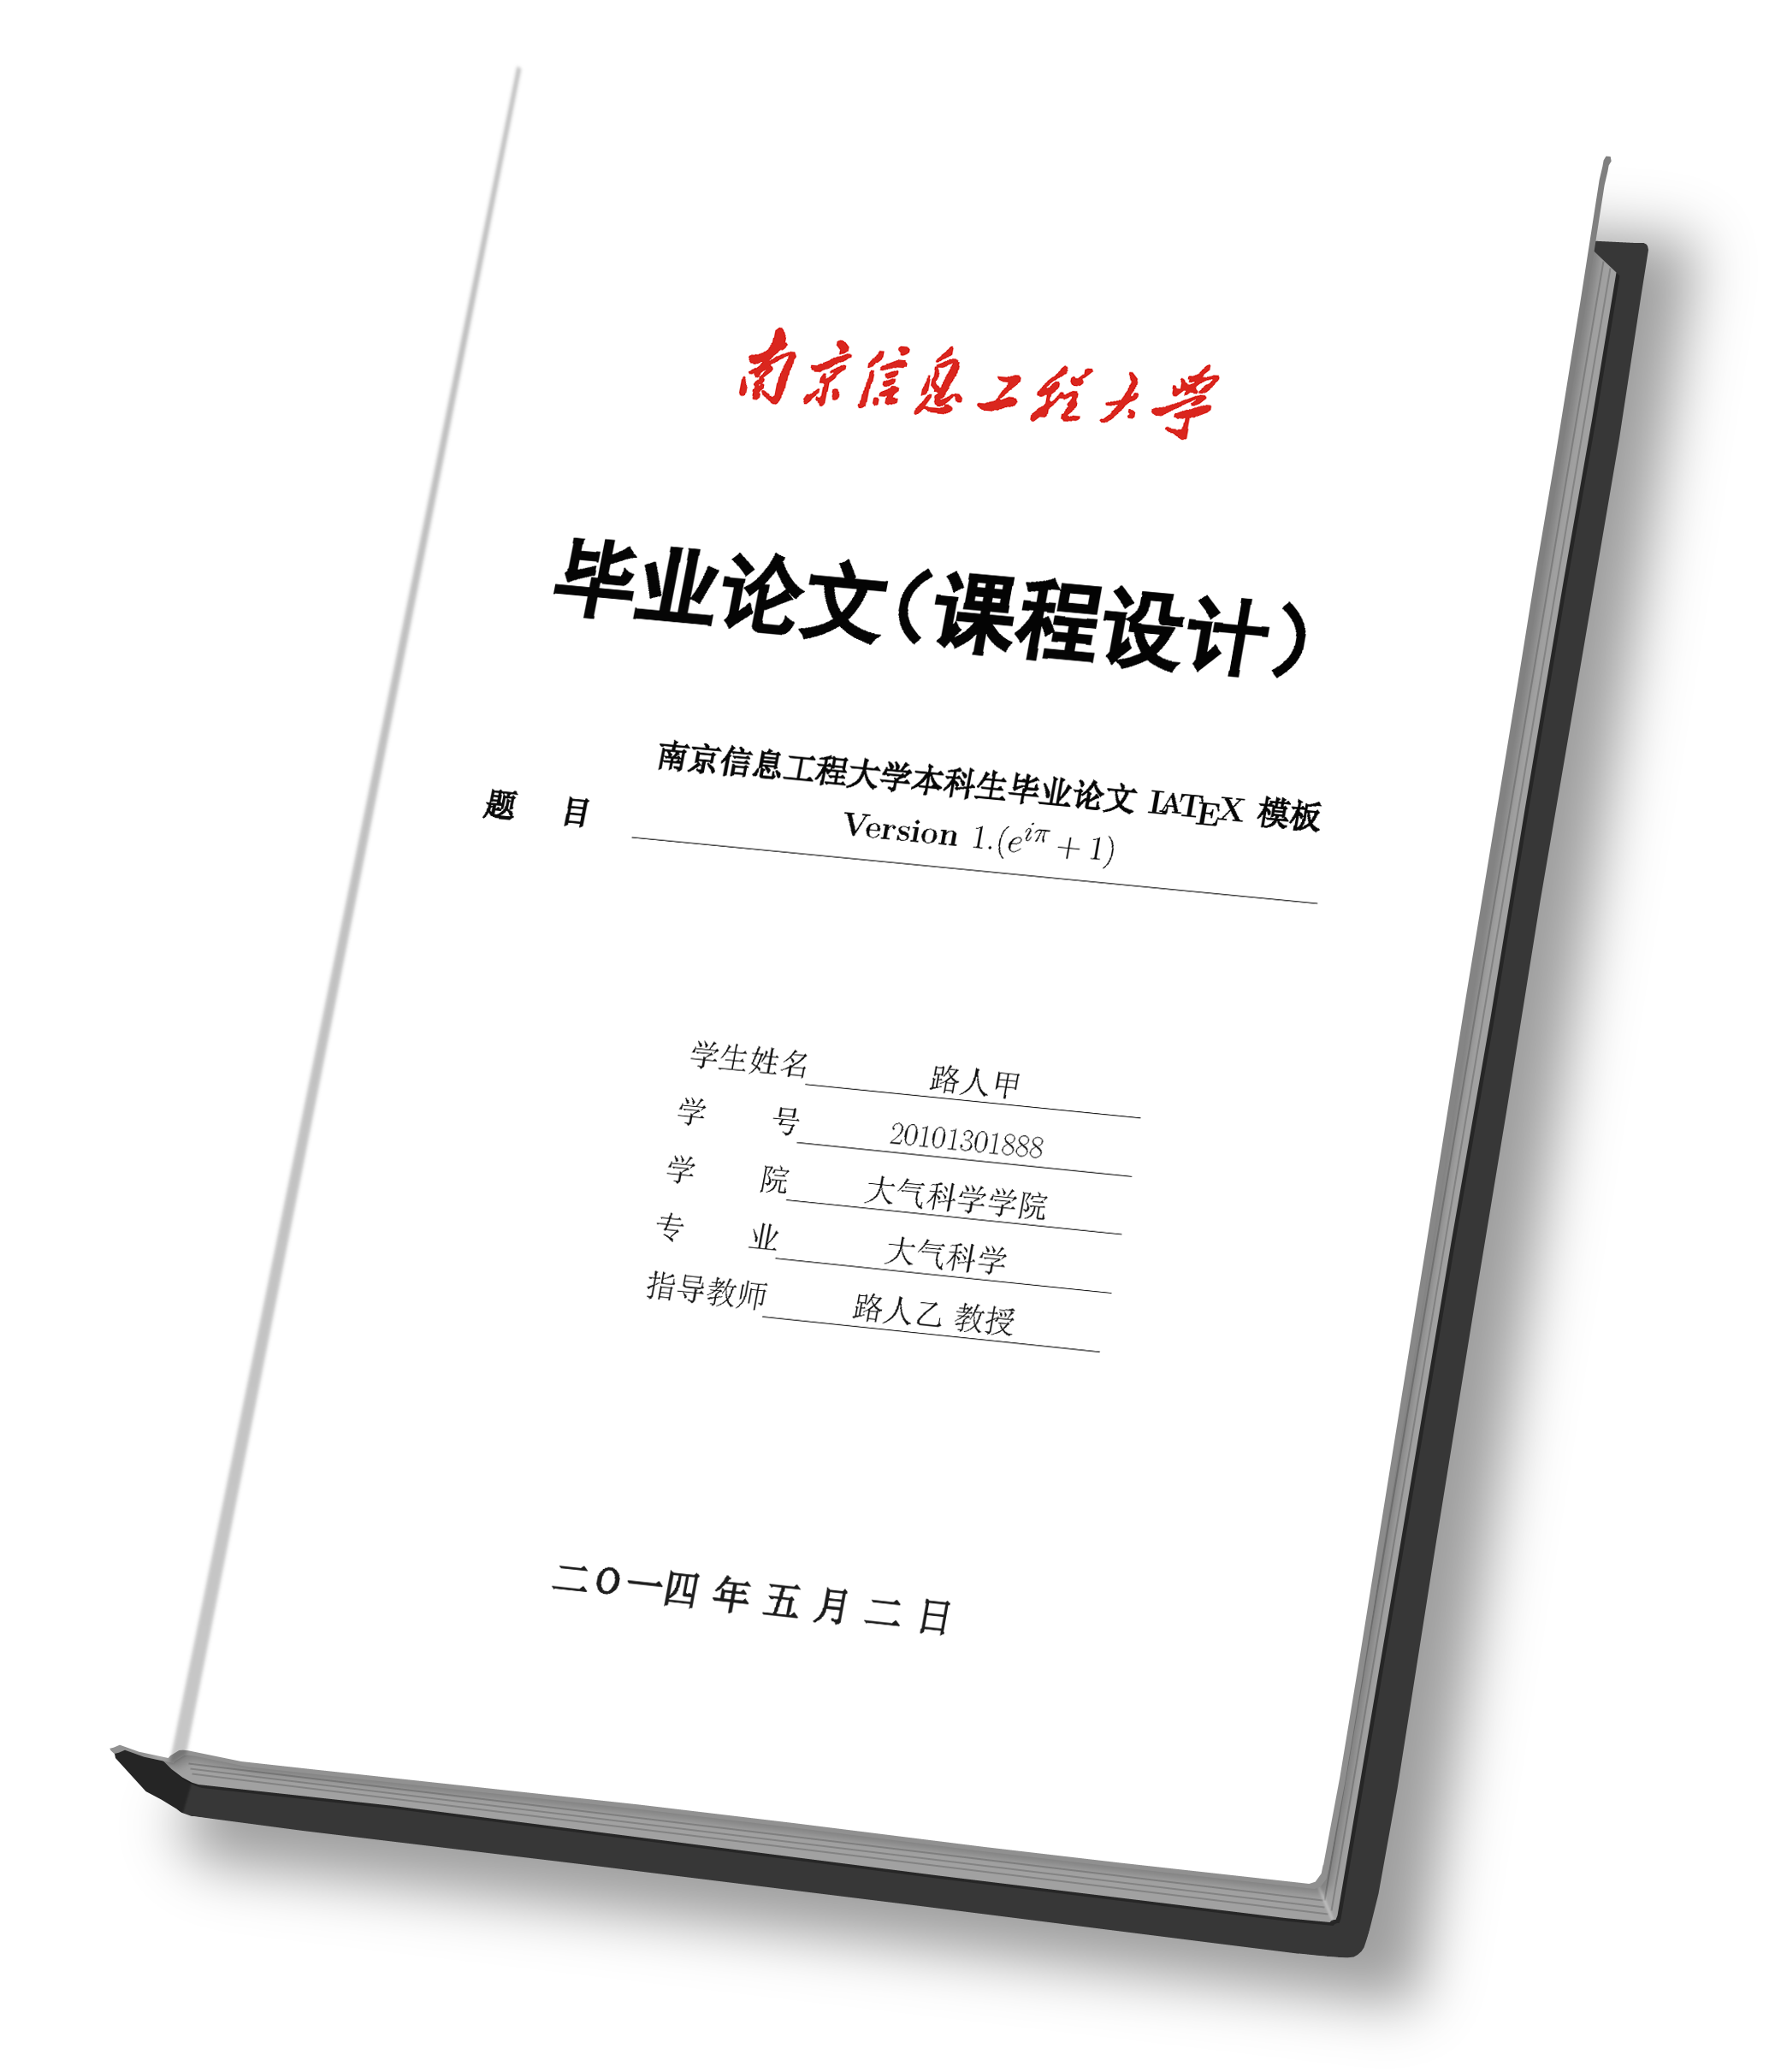
\includegraphics[width=0.6\textwidth]{figs/color/face.png}
\caption{南京信息工程大学本科生毕业论文\LaTeX 模板封面展示}
\label{nuist_face}
\end{figure}

图~\ref{nuist_face}~就是插入到文档中的图片,下面展示一下操作的代码:

{\color{green!50!black}
\begin{lstlisting}[breaklines=true,]
\begin{figure}[htbp!]
\centering
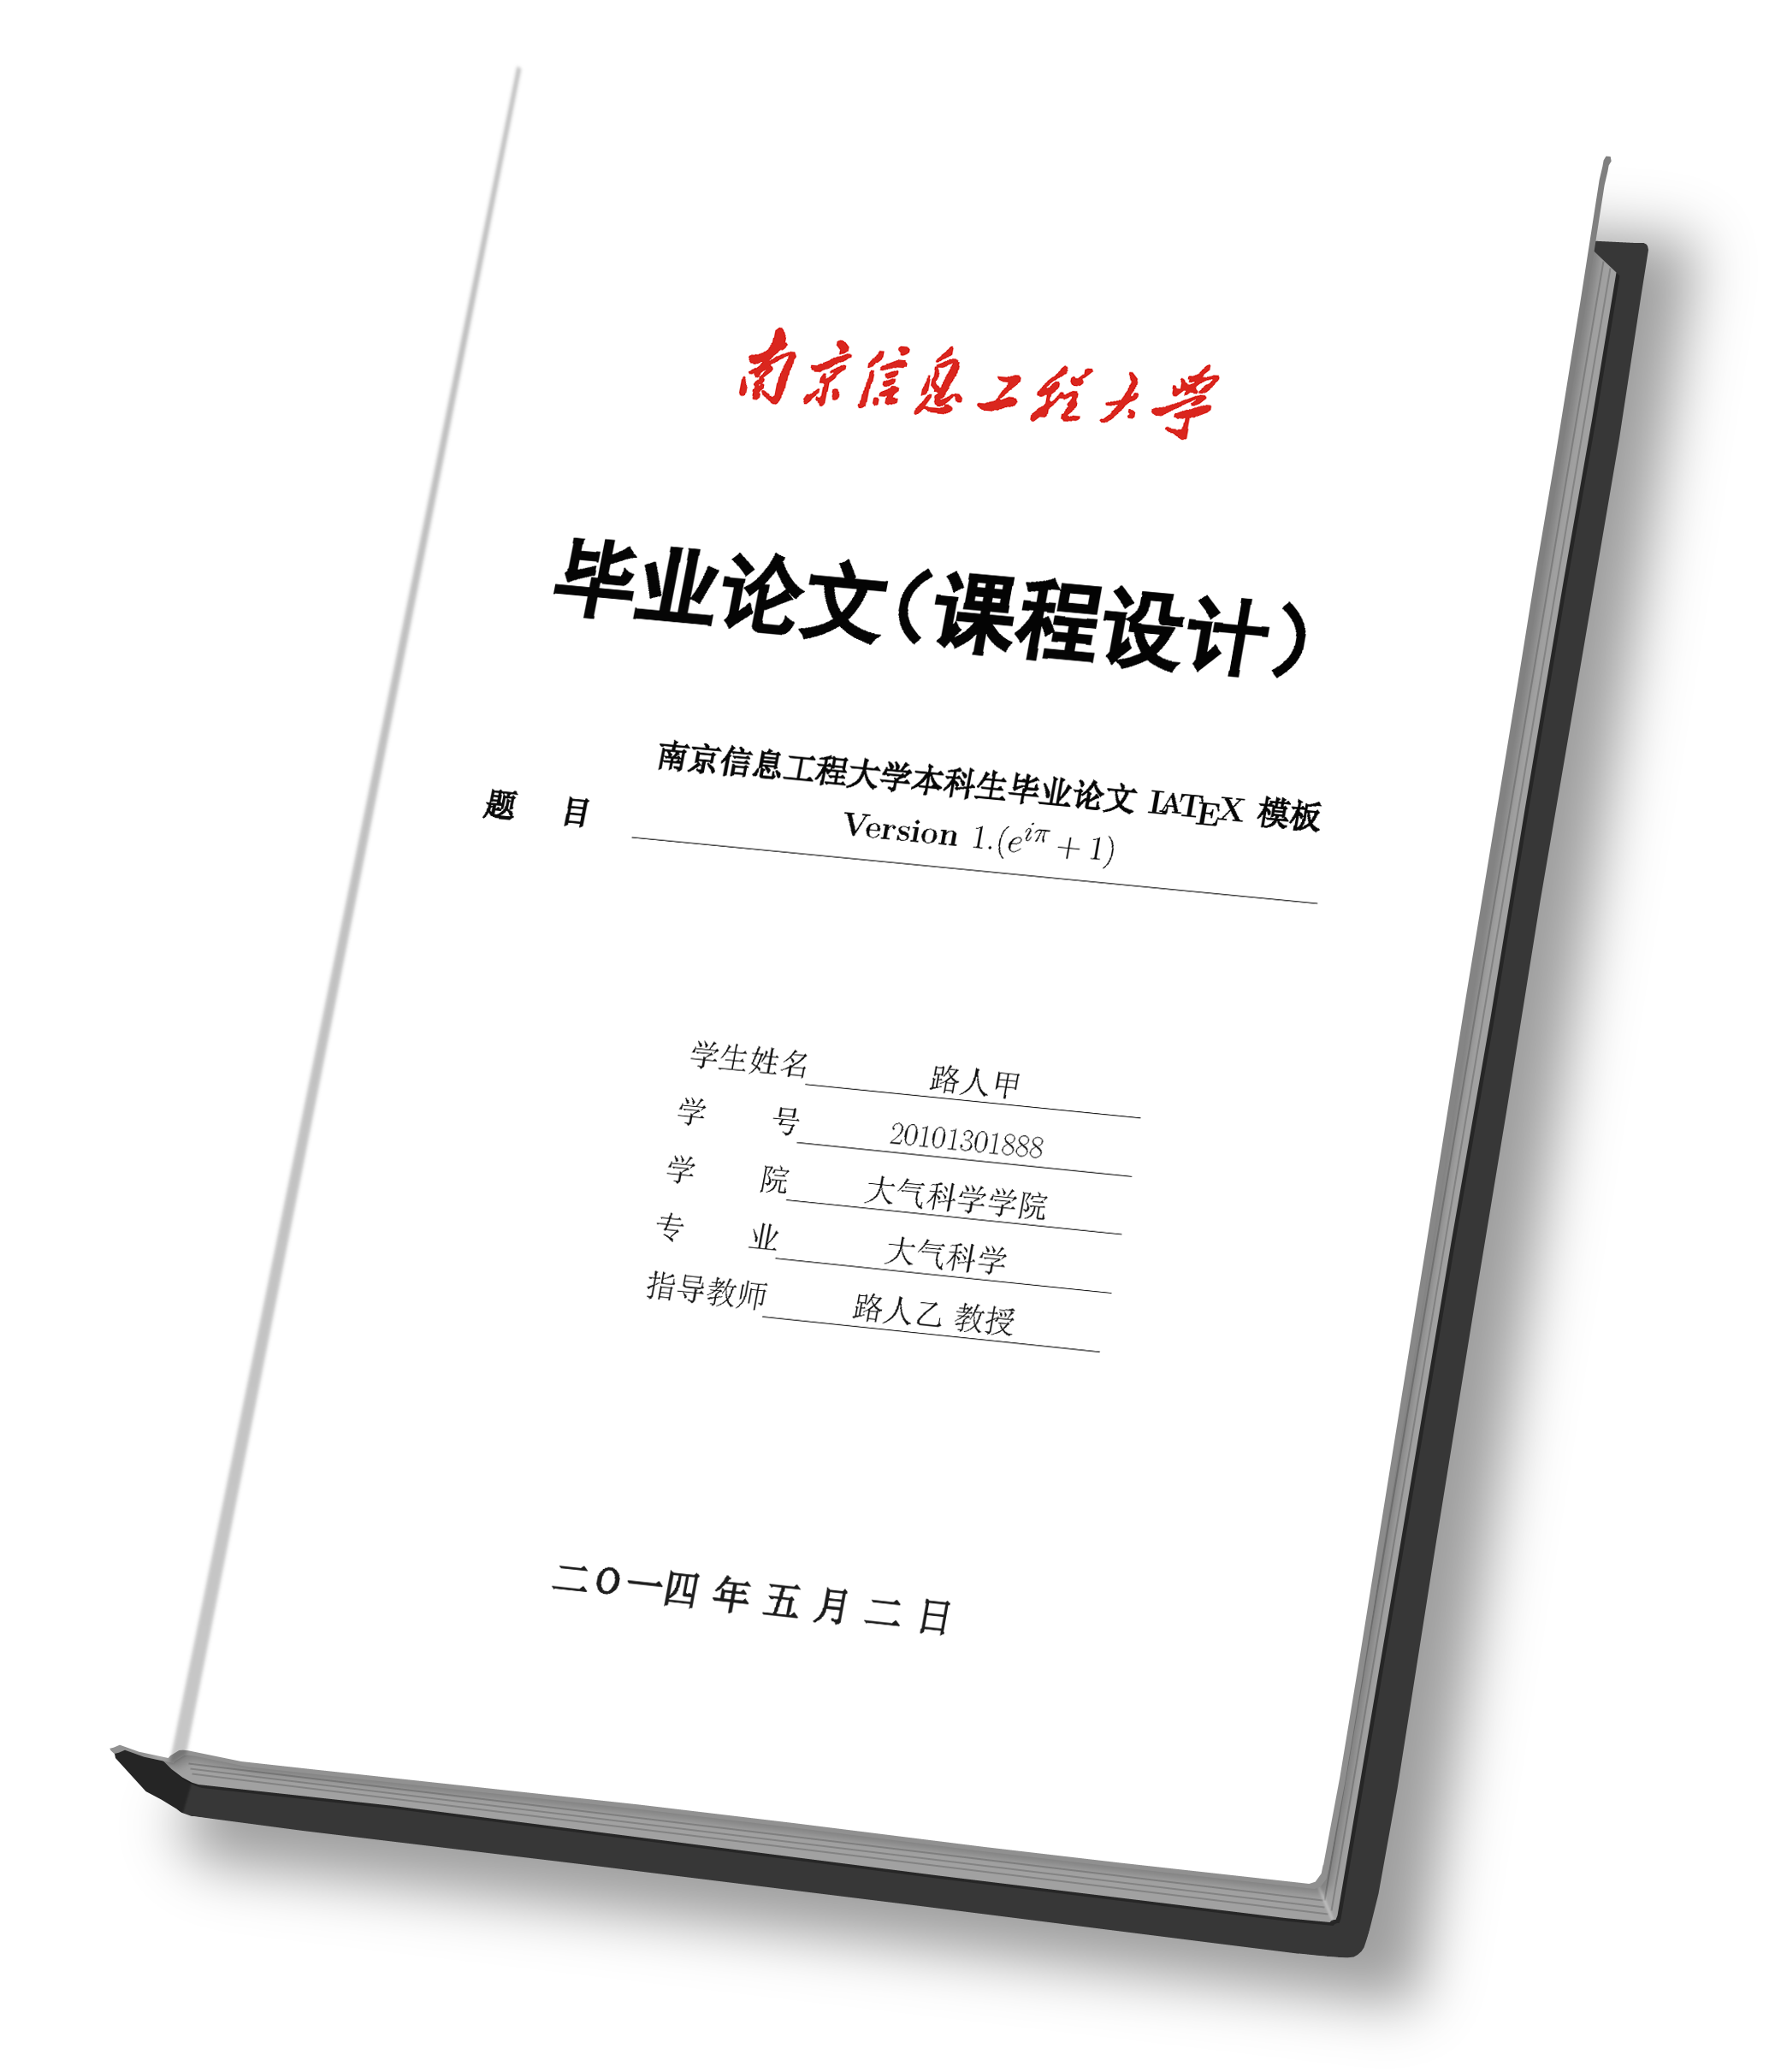
\includegraphics[width=0.6\textwidth]{figs/color/face.png}
\caption{南京信息工程大学本科生毕业论文\LaTeX 模板封面展示}
\label{nuist_face}
\end{figure}
\end{lstlisting}
}
\subsection{并列图及添加子图标题}
大家在做论文时的时候经常需要两幅图并排的情况,还记得在Word用鼠标一点点的拖动吗,通常拖到最后两幅图安排得还是不尽如人意,就算搞定了一组,下一组又要拖呀拉呀的。当然稍稍高明一点可以借助Word的宏命令来控制,但Word中宏的学习曲线十分的陡峭,大家在网上找到的宏,自己想重新定制一下,也是比较困难的。下面来看看\LaTeX 是怎样精确控制并排图片占位大小的,从而使其各占一半水平空间。如图~\ref{cn_map}~:

\begin{figure}[htbp!]
\centering
\includegraphics[width=0.5\textwidth]{figs/color/china1.png}\includegraphics[width=0.5\textwidth]{figs/color/china2.png}
\caption{中国地图展示(左图为素颜,右图为彩妆)}
\label{cn_map}
\end{figure}

其实现代码如下:
{
    \color{green!50!black}
    \begin{lstlisting}[breaklines=true,]
\begin{figure}[htbp!]
\centering
\includegraphics[width=0.5\textwidth]{figs/color/china1.png}\includegraphics[width=0.5\textwidth]{figs/color/china2.png}
\caption{中国地图展示(左图为素颜,右图为彩妆)}
\label{cn_map}
\end{figure}
    \end{lstlisting}
}
是不是感觉图~\ref{cn_map}~的标题不太专业,也想给左右两个子图各加一个标题?那其实也很简单,只要引入subfigure宏包就可以实现。实现后效果如图~\ref{subfig_cn_map}~:

\begin{figure}[htbp!]
\centering
\subfigure[素颜\label{fig:sub1}]{\includegraphics[width=0.5\textwidth]{china1.png}}\subfigure[彩妆\label{fig:sub2}]{\includegraphics[width=0.5\textwidth]{china2.png}}
\caption{中国地图展示}
\label{subfig_cn_map}
\end{figure}

当然我们在引用的时候,可以引用母图,如图~\ref{subfig_cn_map}~,也可以引用子图,如图~\ref{subfig_cn_map}\subref{fig:sub1}~,图~\ref{subfig_cn_map}\subref{fig:sub2}~。

好了让我们来看实现的代码吧:

{\color{green!50!black}
\begin{lstlisting}[breaklines=true,]
\begin{figure}[htbp!]
\centering
\subfigure[素颜\label{fig:sub1}]{\includegraphics[width=0.5\textwidth]{china1.png}}
\subfigure[彩妆\label{fig:sub2}]{\includegraphics[width=0.5\textwidth]{china2.png}}
\caption{中国地图展示}
\label{subfig_cn_map}
\end{figure}
\end{lstlisting}
}

最后再给出一个例子,例如大家在做EOF分析时,可能要两个模态之间进行对比,我们知道每一个模态场都有一个时间序列与其对应,所以这样我们还可能用到$2\times 2$形式的图片排列方式,如图~\ref{fig:eof_12}~。

\begin{figure}[htbp]

\center
\subfigure[第一模态]{\label{eof_1}
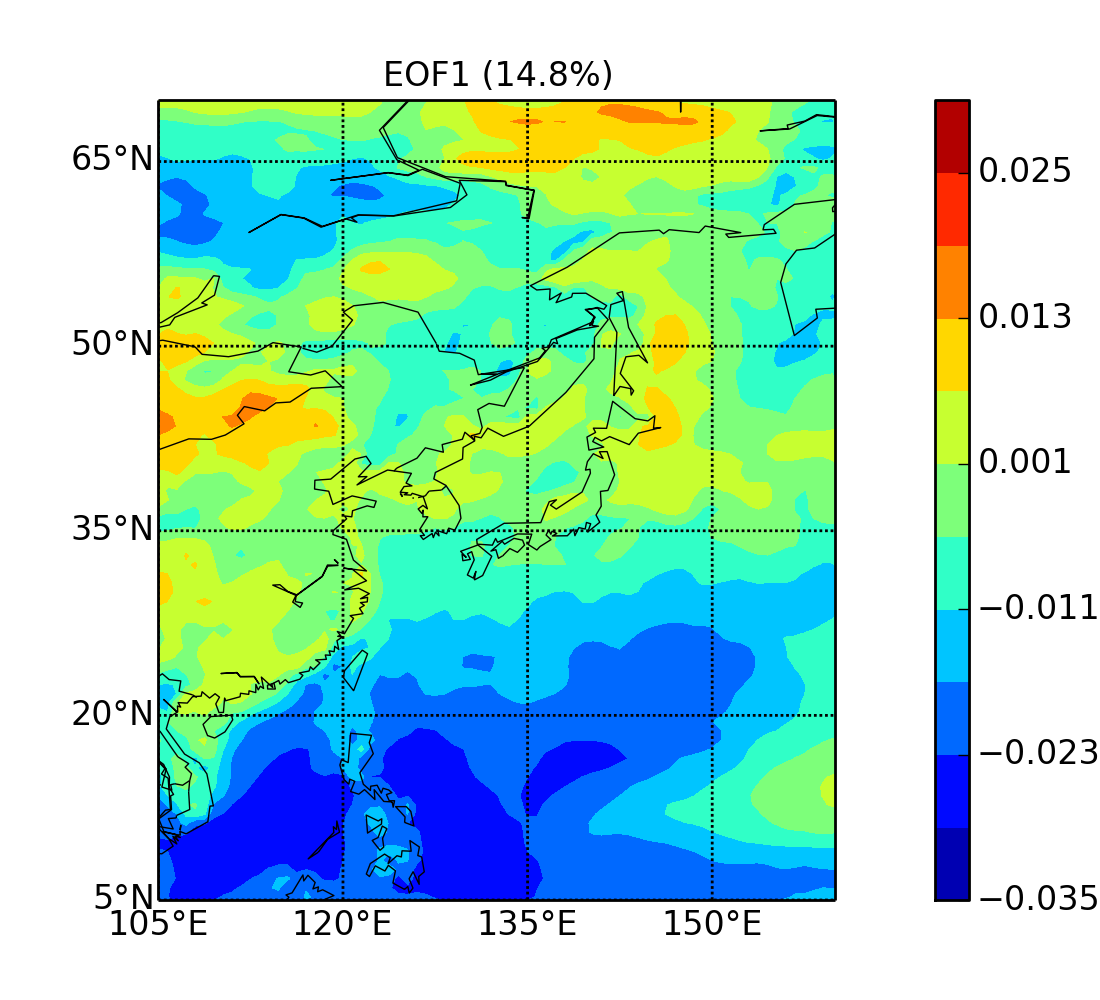
\includegraphics[width=0.4\textwidth]{eof1.png}
}\subfigure[第二模态]{\label{eof_2}
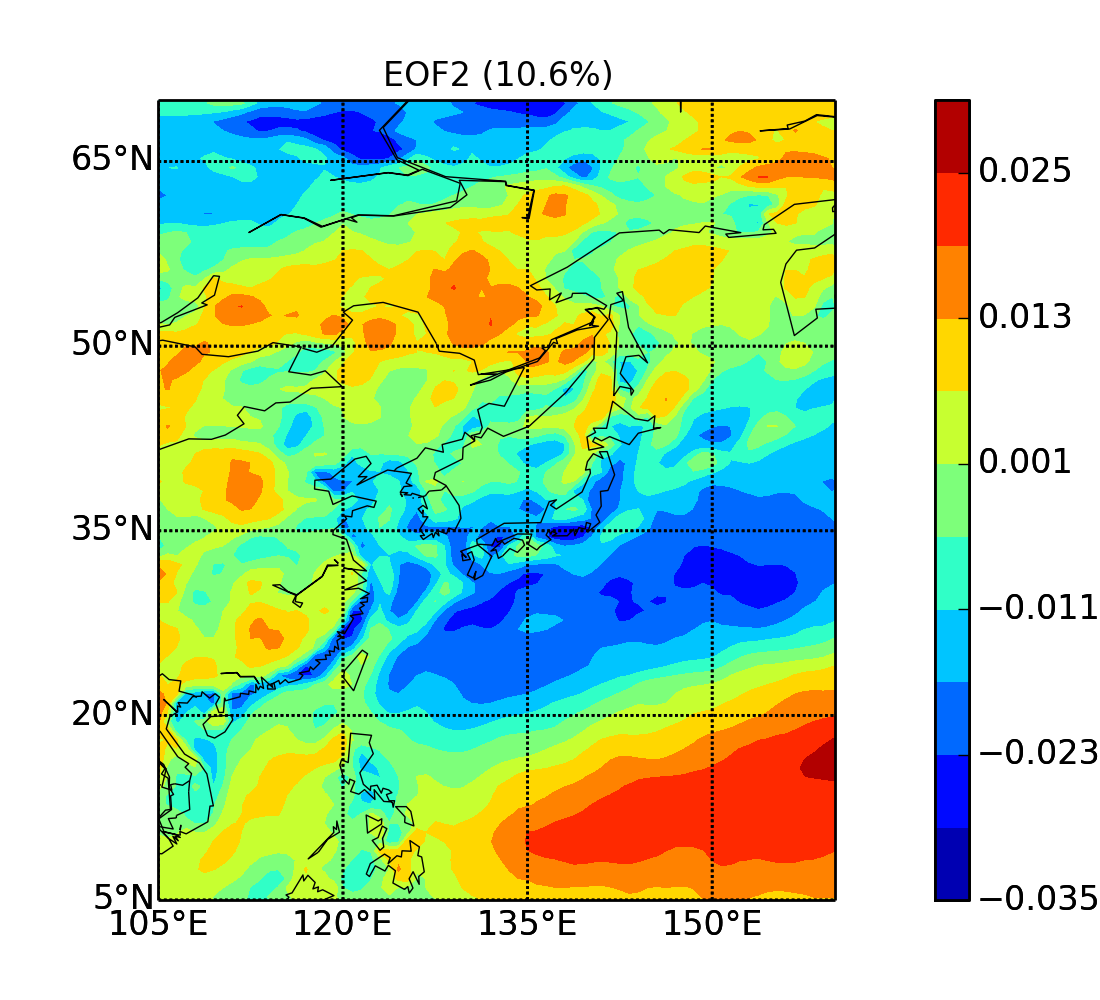
\includegraphics[width=0.4\textwidth]{eof2.png}
}
\\
\subfigure[第一模态对应的时间系数]{\label{eof_t1}
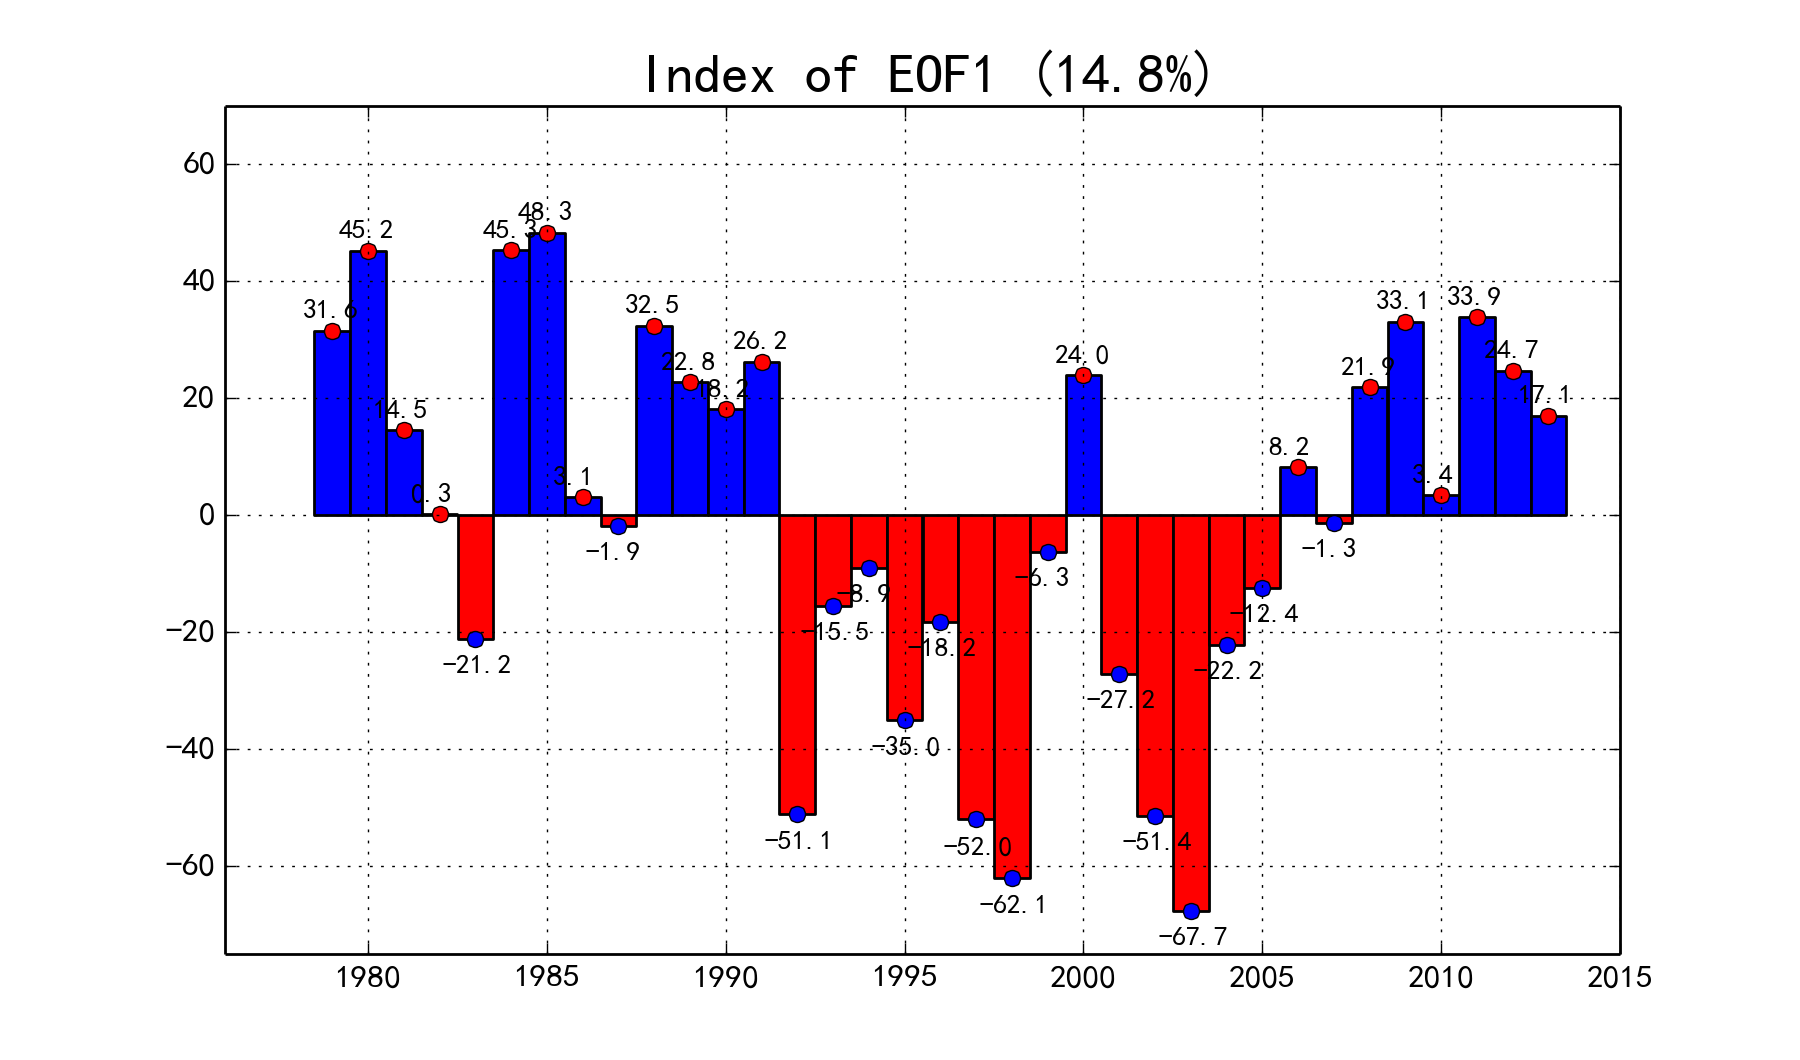
\includegraphics[width=0.4\textwidth]{t1.png}
}\subfigure[第二模态对应的时间系数]{\label{eof_t2}
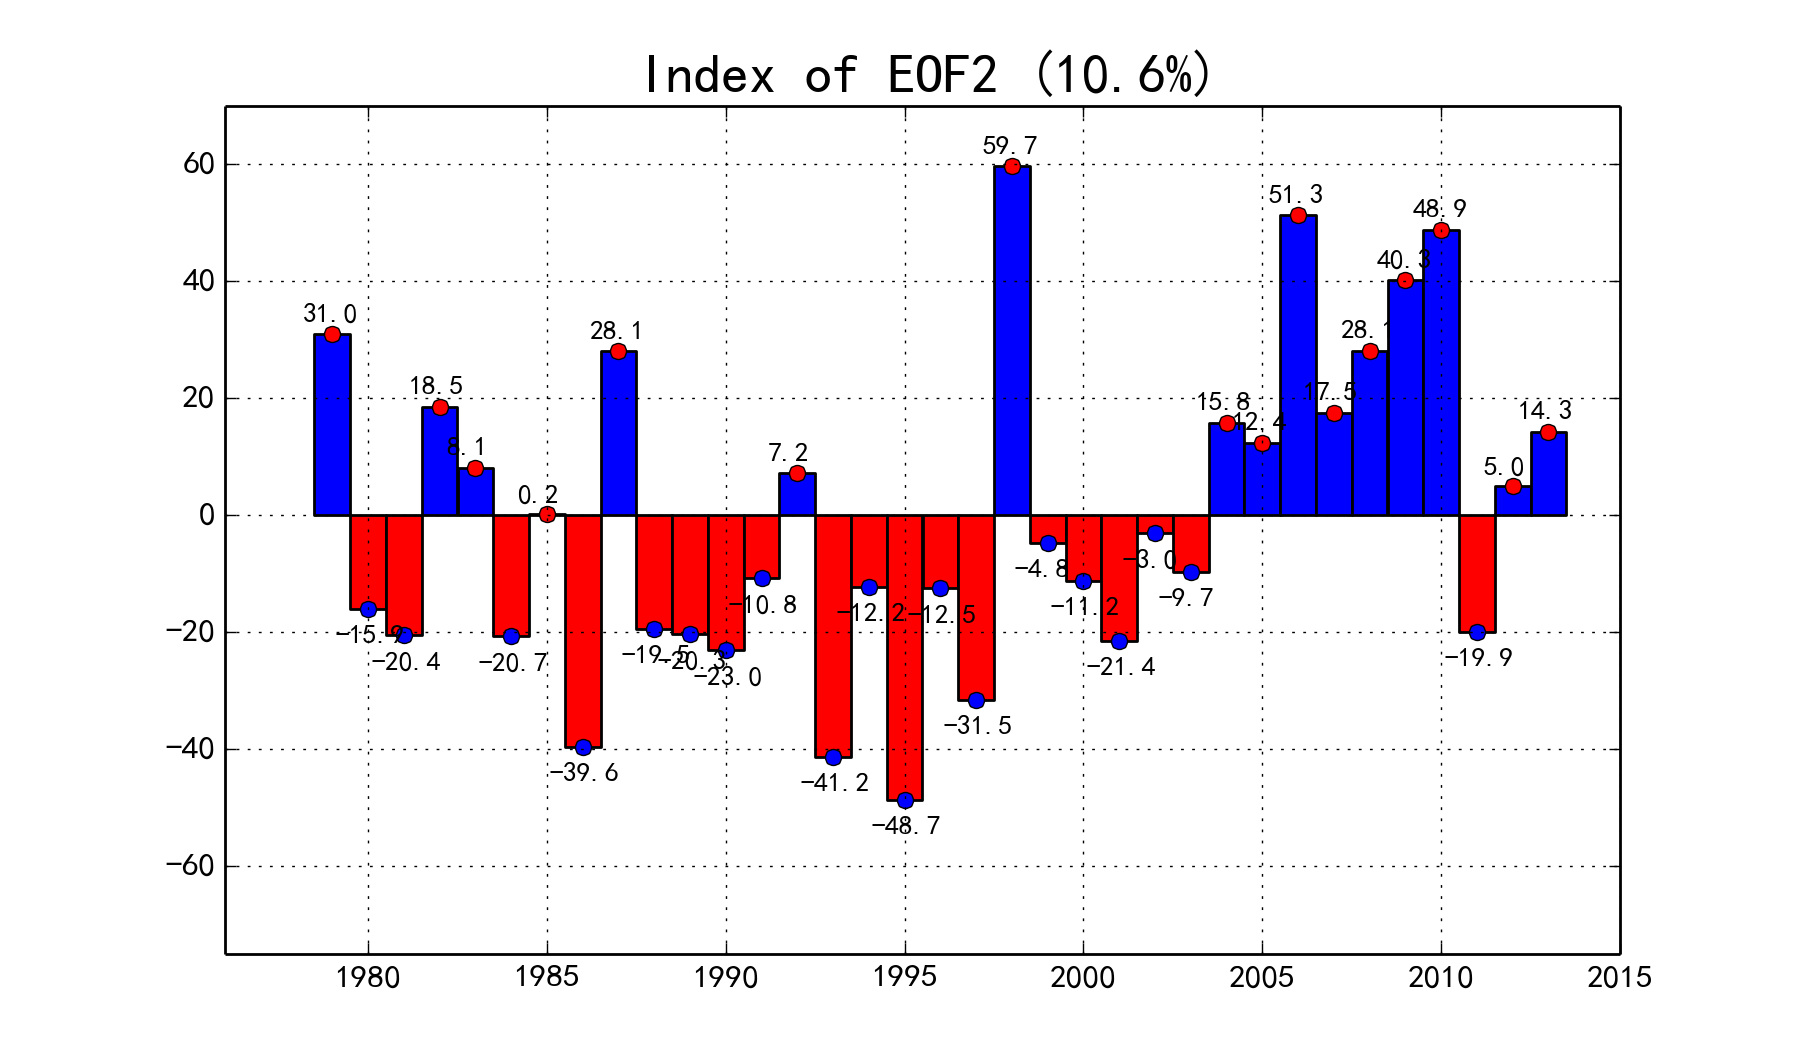
\includegraphics[width=0.4\textwidth]{t2.png}
}
\caption{ABLH的EOF分析结果(第一第二模态及其时间系数)}\label{fig:eof_12}
\end{figure}

我们可以用下面的命令来实现:

{\color{green!50!black}
\begin{lstlisting}[breaklines=true,]
\begin{figure}[htbp]
    \center
    \subfigure[第一模态]{\label{eof_1}
    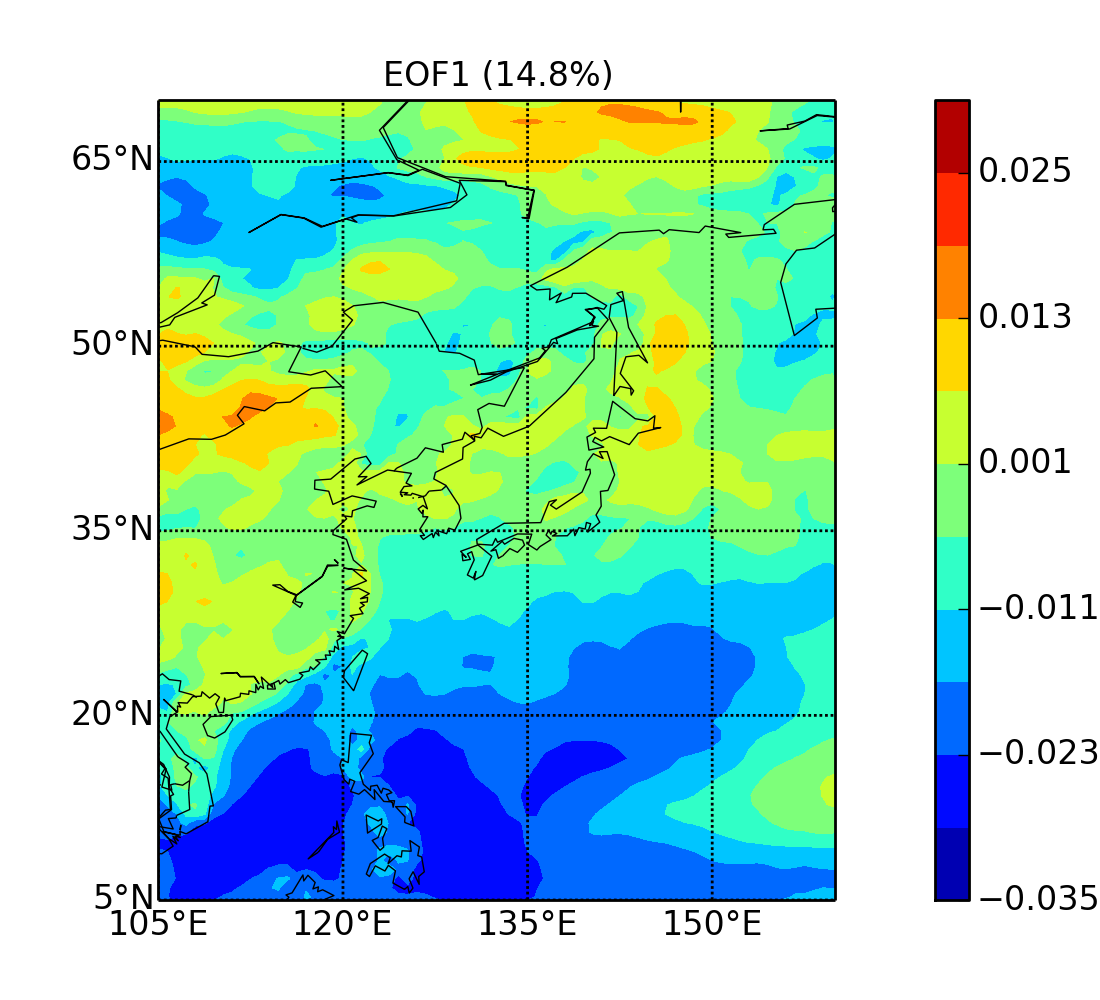
\includegraphics[width=0.4\textwidth]{eof1.png}
    }\subfigure[第二模态]{\label{eof_2}
    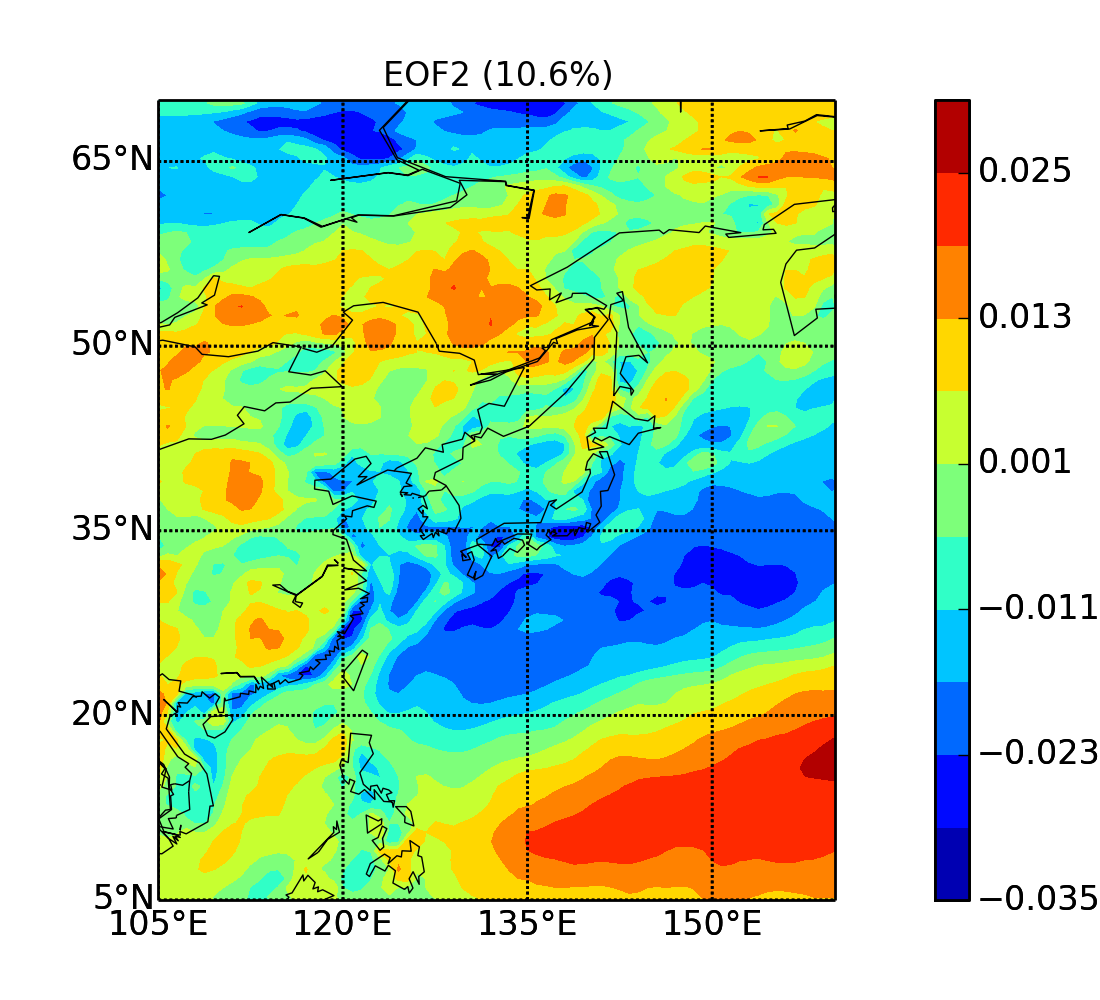
\includegraphics[width=0.4\textwidth]{eof2.png}
    }
    \\
    \subfigure[第一模态对应的时间系数]{\label{eof_t1}
    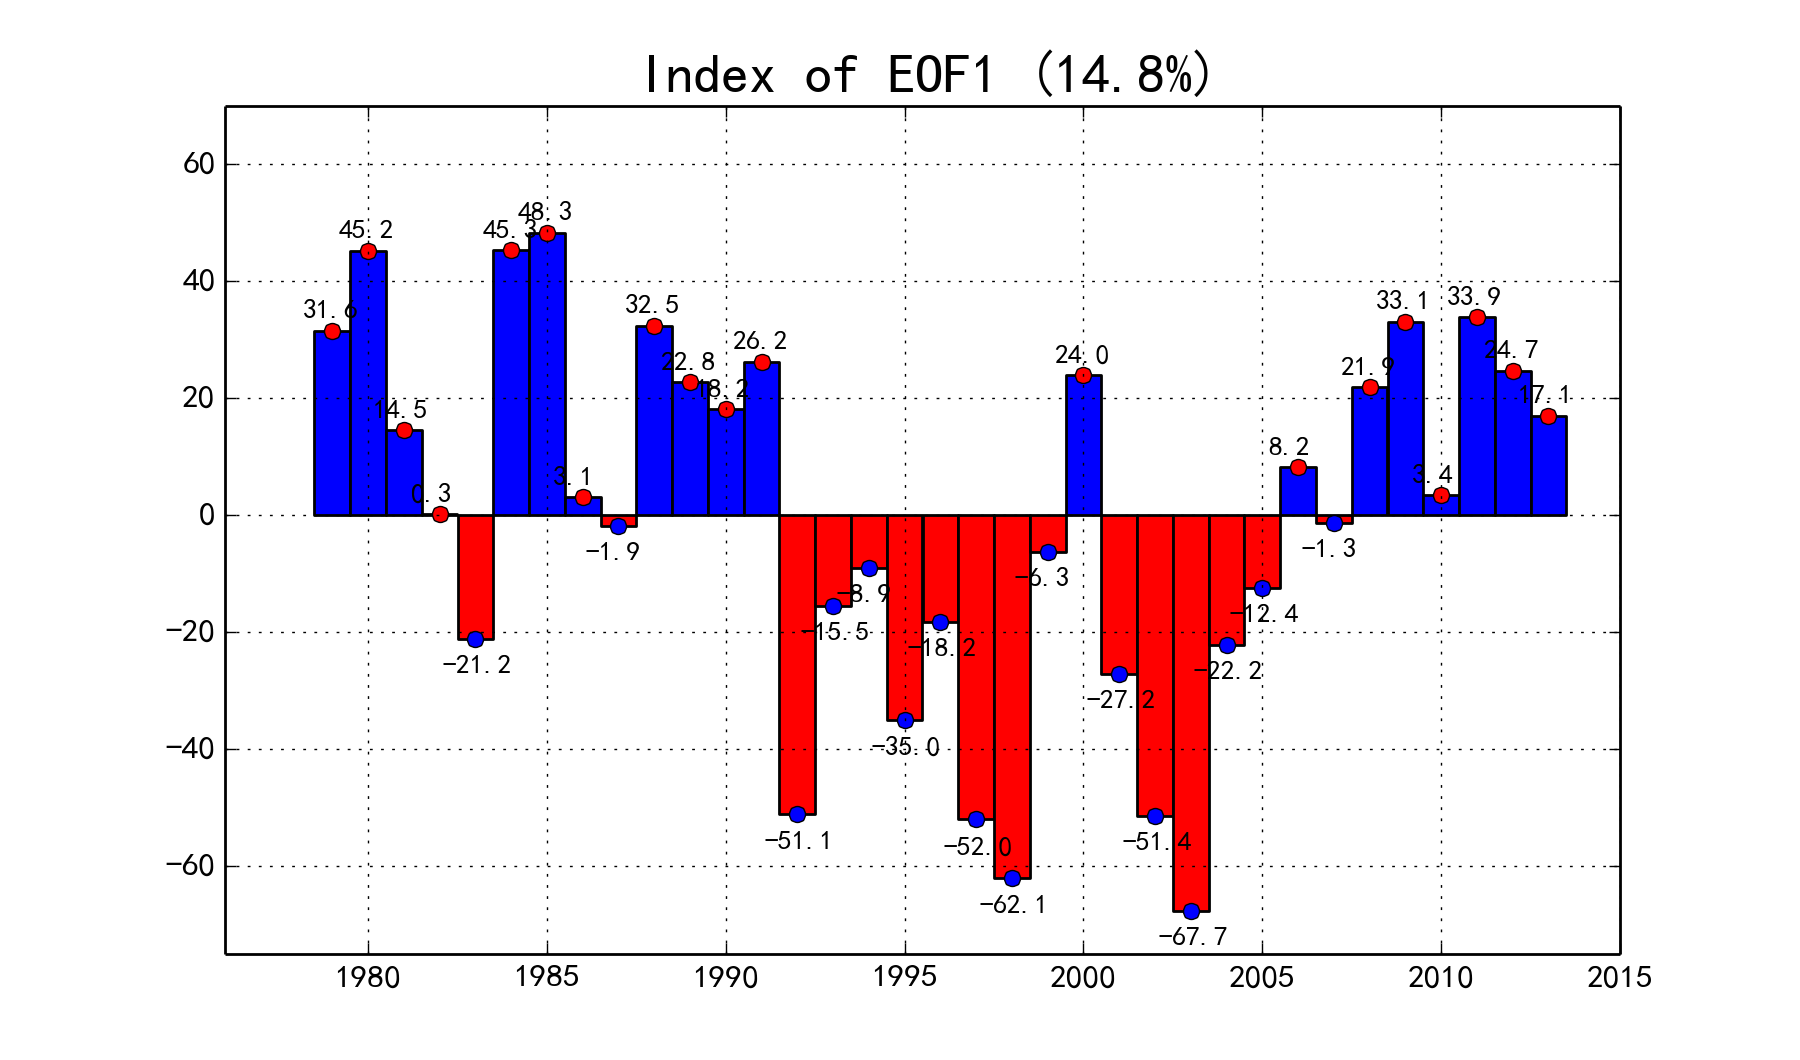
\includegraphics[width=0.4\textwidth]{t1.png}
    }\subfigure[第二模态对应的时间系数]{\label{eof_t2}
    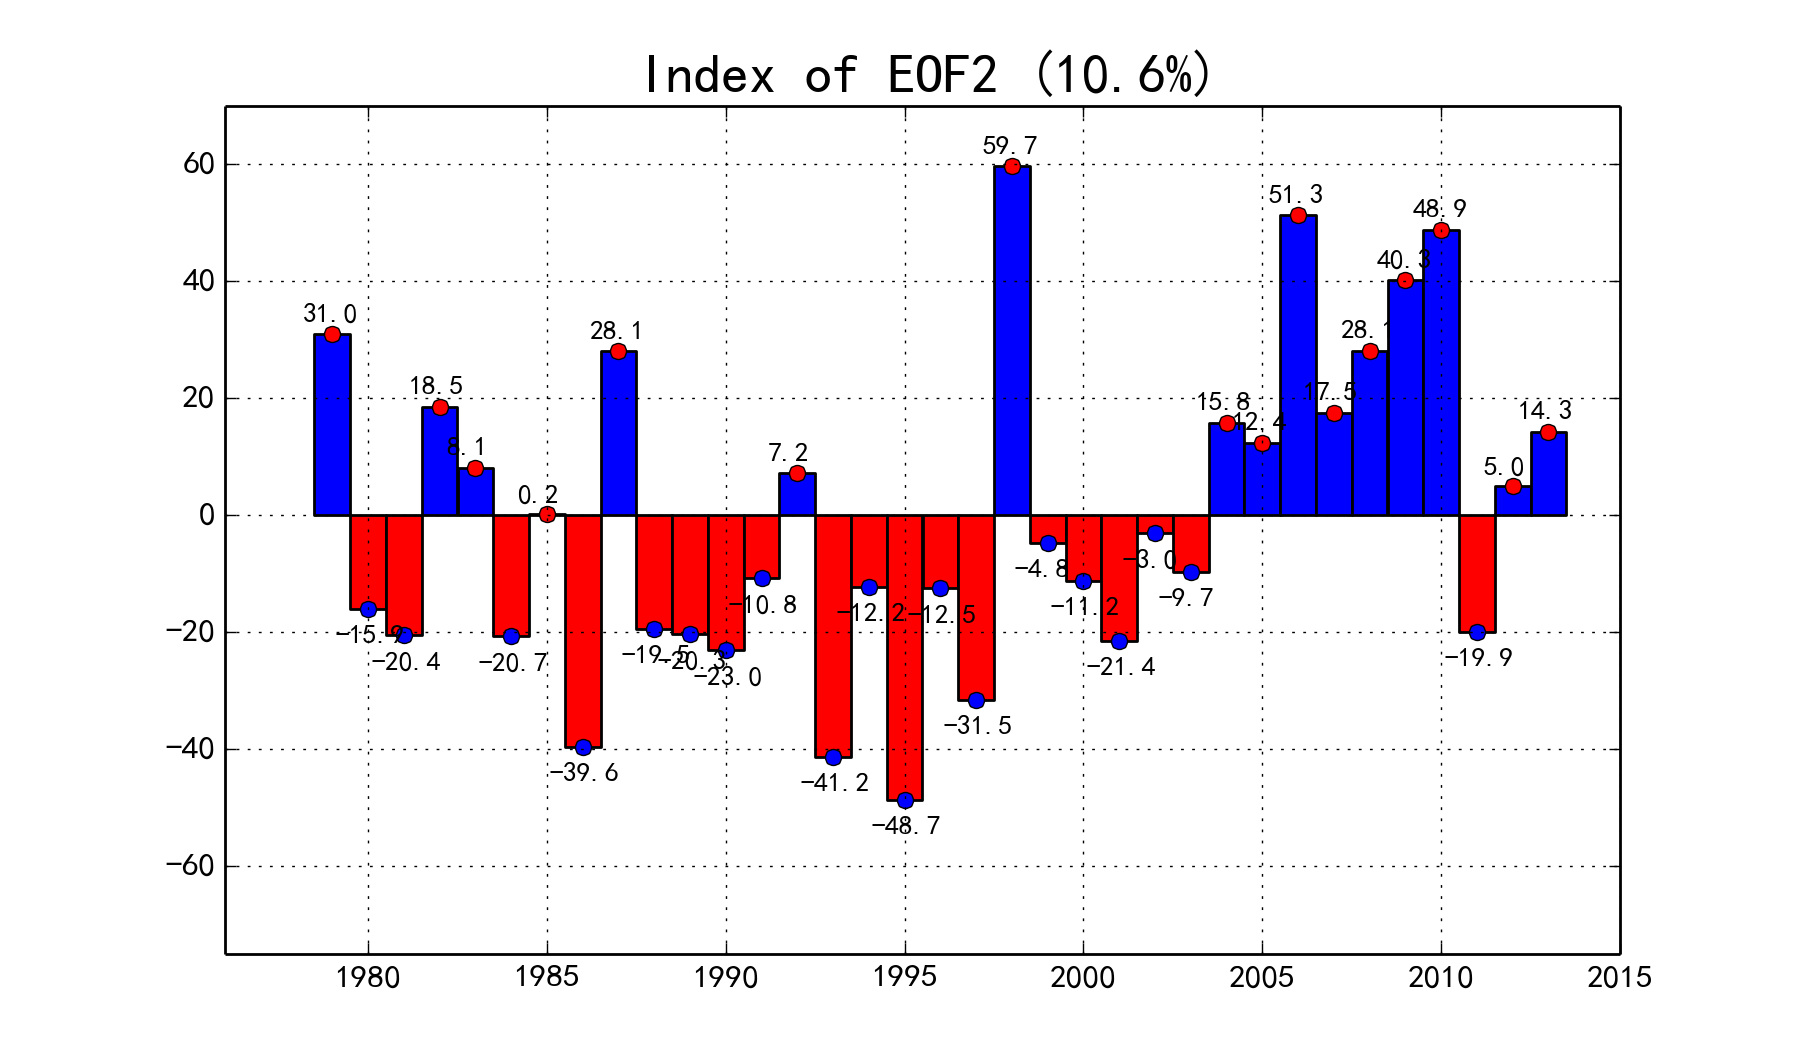
\includegraphics[width=0.4\textwidth]{t2.png}
    }
    \caption{ABLH的EOF分析结果(第一第二模态及其时间系数)}\label{fig:eof_12}
\end{figure}
\end{lstlisting}
}

朋友们应该也发现奥秘所在了,对,就是那个双斜线$ \backslash\backslash$的作用,双斜线在\LaTeX 排版系统中就是换行的命令,知道了这一点,大家可以随意安排自己的图片了,可以用$2\times 3$或者$3\times 2$来摆放自己插图了。


\subsection{图片文件夹的指定}
细心的朋友可能会发现生成~\ref{subfig_cn_map}~和图~\ref{cn_map}~所用的代码在指定图片路径时的写法不同,一种是相对路径,另一种是只有图片名称。这是为什么呢?原因很简单。为了在写作时引用图片方便,本文在导言区写上这样的\verb|\graphicspath{{figs/color/}}|一名命令,来宏观地指定图片所存放的位置。

这一功能的好处就是,对于有的同学电子文档和打印文档所用图片色彩格式不同,这样只要一条命令就可以切换到另一个文件夹了,比较实用。

\section{排版表格}
\LaTeX 中生成简单的表格还是比较方便的,可以用tabular 环境来实现。下面就来做一个论文中经常用到的三线表,如表~\ref{table_1}~。

\begin{table}[htbp!]
\centering
\caption{本模板中部分使用的宏包及功能}\label{table_1}

\begin{tabular}{ccccccccc}
\whline 
宏包名称 & amsmath&caption&geometry&ulem&xcolor&setspace&hyperref \\ 
\hline 
作用 & 数学公式&定制标题&页面设置&下划线&颜色&行距&超链接 \\ 
\whline 
\end{tabular}
\end{table}

其实现代码如下:
{\color{green!50!black}
\begin{lstlisting}[breaklines=true,]
\begin{table}[htbp!]
\caption{本模板中所用的宏包及功能}\label{table_1}
\begin{tabular}{ccccccccc}
\whline 
宏包名称 & amsmath&caption2&geometry&ulem&xcolor&setspace&hyperref&titletoc \\ 
\hline 
作用 & 数学公式&定制标题&页面设置&下划线&颜色&行距&超链接&目录样式 \\ 
\whline 
\end{tabular}
\end{table}
\end{lstlisting}
}
如果表格比较长,那就要用到跨页表格排版宏包longtable了(模板中已引入该宏包)。基本的表格排版情况就介绍这么多,大家感兴趣自己慢慢去探索吧。
\section{排版代码}

本模板使用listings宏包排版代码,效果如下:
\begin{lstlisting}[breaklines=true,language=Python]
    # Hello World!
    print('Hello World!')
\end{lstlisting}

其实现代码如下:
\begin{tcblisting}{listing only,boxrule=-1pt,colback=white}
\begin{lstlisting}[breaklines=true,language=Python]
    # Hello World!
    print('Hello World!')
\end{lstlisting}
\end{tcblisting}

如果代码中注释有中文,\XeLaTeX{} 会警告系统中的仿宋字体不支持斜体,这个问题有待解决。

listings支持的语言相对有限,如果需要更好的语法高亮效果,可以考虑使用minted宏包。模板目前尚未实装该宏包,感兴趣的话可以参考\url{https://zhuanlan.zhihu.com/p/348850937}。
\section{排版参考文献及引用}
\subsection{使用bibliography排版参考文献}
编写参考文献一章是个很无聊的工作,且工作量不小。使用“GB/T 7714—2015 BibTeX Style”排版参考文献可以省去模板用户研究参考文献排版规范的时间。尽管知网提供GB/T 7714—2015格式引文,但是知网提供的引文其实存在一个小问题:标点后没有空格,需要我们自行添加空格(知网外文文献提供的可供复制的引文做的更差,居然敢说是GB/T 7714—2015格式的……)。至于外文文献,引文基本上需要我们对照规范自行编辑。将参考文献排版工作交给程序,将我们从这个无聊且耗时的工作中解放出来。

模板用户需要编辑bibliography.bib文件,填写参考文献的各项属性,如title、author、year等,具体请参考\url{https://github.com/CTeX-org/gbt7714-bibtex-style#%E6%96%87%E7%8C%AE%E7%B1%BB%E5%9E%8B}。OVERLEAF网站对bibtex有比较详细的解释,如果您想要了解关于bibliography文件的基本知识,请参考\url{https://www.overleaf.com/learn/latex/Bibliography_management_with_bibtex#The_bibliography_file},其它关于bibtex的问题也可以参考该网站。其实bib文件的生成工作也可以交给文献管理软件,进一步实现参考文献管理自动化。

bib文件示例:
{\color{green!50!black}
\begin{lstlisting}[breaklines=true,]
    @online{x1,
    title = {The Not So Short Introduction to LaTeX2e},
    year = {2021},
    author = {Tobias, O and Hubert, P and Irene, H and Elisabeth, S},
    url = {http://tug.ctan.org/info/lshort/english/lshort.pdf},
    urldate = {2021-06-05},
    langid = {english},
  }
  
  @book{x2,
    title = {LaTeX2e 及常用宏包使用指南},
    author = {李平},
    date = {2004},
    publisher = {{清华大学出版社}},
    location = {{北京}},
    langid = {中文;}
  }
\end{lstlisting}
}
示例中的x1、x2为参考文献的标识符,可以随意设定,在正文中使用\verb|\cite{x1}|命令即可实现文献交叉引用。

bib文件编辑完成后,用户需要依次进行下面四个操作:编译文档、在命令行环境执行bibtex命令、编译文档、编译文档。在Visual Studio Code中操作为:
\begin{enumerate}[1、]
    \item 点击\TeX 插件中的“Build LaTeX project”
    \item 在VSC的TERMINAL中执行“bibtex 文件名.aux”,如“bibtex NUIST\_thesis.aux”
    \item 点击\TeX 插件中的“Build LaTeX project”
    \item 点击\TeX 插件中的“Build LaTeX project”
\end{enumerate}
如果想了解原理,请参见\url{https://liam.page/2016/01/23/using-bibtex-to-generate-reference/}。用户也可以自行为\TeX 插件添加新的Recipe,一键完成编译。

若参考文献发生变更,或是编译发生错误,用户需要先清除.aux, .bbl, .blg文件后,重新执行以上操作。

学校规定的参考文献排版规范有一点与国标不同:我校要求英文人名仅首字母大写。这要求模板用户在执行bibtex命令后,修改生成的bbl文件,将其中的英文人名改为符合我校要求的首字母大写、其余字母小写。

{\color{blue}
2022-01-10:更新bib样式gbt7714-2005-numerical.bst,已实现仅首字母大写、其余字母小写。经考证,姓氏字母全部大写的要求是gbt7714-2015版中的修改,而按学校要求使用gbt7714-2005版格式,则只有首字母大写。\cite{陈浩元2015GB}}

\subsection{(已弃用)thebibliography环境排版参考文献}
注释掉nuist.cls文件的第50行至第52行,并取消注释第55行至第57行,来启用thebibliography。

使用thebibliography环境来排版参考文献,代码如下:
{\color{green!50!black}
\begin{lstlisting}[breaklines=true,]
\begin{thebibliography}{99}\setlength{\itemsep}{-0.1mm}
\begin{spacing}{1.2}
\zihao{-5}
\bibitem{x1}The Not So Short Introduction to 
\LaTeX2e \ by Tobias Oetiker, Hubert Partl, Irene Hyna and Elisabeth Schlegl.
\bibitem{x0}李平.\LaTeX2e 及常用宏包使用指南[M].清华大学出版社,2004.
\bibitem{x3}罗振东,葛向阳.排版软件\LaTeX 简明手册[M].第二版.北京:电子工业出版社,2003.
\end{spacing}
\end{thebibliography}
\end{lstlisting}
}
引用文献条目时使用\verb|\ucite{}|命令,例如代码\verb|\ucite{x1}|和\verb|\ucite{x2}|就可以产生\cite{x1}和\cite{x2}上标。
%%% 正文部分

\section{写在后面(第一版作者)}

时间过得真快,从五一动手,到码字码到这里差不多快三天了。这么短的时间,不管模板本身还是说明文档肯定还是不够完善的。但时间所迫,也必须到这了。

有人也许行会产生疑问,word不是用着挺好的吗,干嘛要学这个,干嘛要用这个写论文呢?其实要我回答呢,的确是这样的,随便用哪个排版软件用顺手了就好了,没人强迫你做什么,关键在于自己是怎么想。

去年笔者在写学年论文时,就“吃了亏”,先是用\LaTeX 写的,生成的pdf格式的文档,但是最后学院不认,说必须用word版的,无奈后来又用word重排了一遍。(所以这里插一句,如果真有哪位朋友想用这个模板,请“严重”地考虑这个“严重”的后果,弄不好到最后,只能用它排个打印版玩玩,电子版还得word 去。)

而对笔者来说,无所谓,不是天空经常会飘来五个字儿,叫“这都不是事儿”嘛,人生本就是向死之生,要是总走直线,太快到终点了怎么办?所以人生的要义就在于走“弯路”,走得越“弯”走得越长嘛。

\section{第二版修订说明}
\subsection{第二版!新鲜出炉!}
两年以后\footnote{第二版修订于2017年3月13日,\url{https://github.com/LirenW/NUIST_thesis_template_V2.0}},这个模板又被重新更新了一次(原作者应该并没有更新过(因为并不能联系到原作者(sigh。因为每年的格式都会进行一些修改,所以按照现在的格式改了一下模板,特别是字号和字体,并且针对一些问题进行了修改(以下如果感觉麻烦可以略过233),不过要注意的是,NUIST一向不欢迎PDF格式的论文提交,因此此模板,正如原作者说的那样,需要慎用、慎用和慎用。\par
对于无法复制PDF的问题,由于CTeX的设置问题解决方案比较复杂,本模板采用修改字体为Adobe Song Std 的方法,不过如果要完整解决此问题请参考\url{https://www.zhihu.com/question/32207411}这个回答,不过低版本的CTeX+WinEdit套装中CTeX版本过低无法使用,可以考虑升级全部宏包(此方法可能会导致WinEdit宏包冲突,慎用)也可以等新版本的套装(听说快出了)。\par
关于行距的问题,虽然word和LaTeX的行距计算方法相同(行距:一行文字的基线(Base Line)到下一行文字的基线的距离,详见\cite{x4}),但是修改出的文章行距感觉比word略宽,不知道为什么,期待后人能解决此问题!\par
\subsection{修订者的话}
说完了专业问题,聊点其他的话题好了。笔者接触LaTeX也蛮久了,从数学建模就用自己修改的模板进行论文写作,到写毕业论文时还是用LaTeX,感觉长文章基本脱离Word了,不是不会用(不自夸地说,论Word排版本人也完全可以完成长文章的各种排版工作),而是感觉Word排出来的东西一点也不美。\par
Knuth感觉自己写的东西被编辑排成了渣,于是很不开心地花时间做了个排版系统;乔布斯觉得手机太丑,于是自己做了个iPhone。我也有这种感觉,且不说Word那蛋疼的贪心断行算法(最常见的例子的是加上了数学公式和英文字符后完全不对齐的右边界)、令人抓狂的图片摆放,就拿最简单的来说,一个写作软件,为什么要让用户找不到如何更新引用!我知道那复杂的域代码和目录生成,然而一个一个设置它们的格式实在令人发指,并且一个不小心,版面就跑到十万八千里以外。不过什么是美呢?想来对我来说的话就是“Simple is the best”,能让电脑自动计算的事情完全不应该由手工来做,能动脑解决的就绝不动手。\par
世界是因为懒人才变得舒适,但“懒”往往需要的是Critical Thinking和Curiosity,而对我来说,对美这一形而上的终极目标的追求促使我探索这个世界,而对这个世界无穷无尽的美好的好奇让我在探索的过程中不太无聊。\par
引用百度百科(好吧我最唾弃百度的各种玩意了)TeX的词条的一句话吧:
\begin{quote}
  TeX是一种乐趣: 使用TeX不仅仅是一种工作手段,也是一种乐趣。它有挑战,也有荣誉。很多人在熟悉了TeX之后都开始把使用TeX作为一种爱好,而不是一件枯燥无味的劳动。
\end{quote}
我使用TeX就是因为它简洁明快,让我专注于内容而不需要纠结于无聊的排版疏忽,随意调节结构而不用担心随之而来的格式更新,总而言之就是这个样子\footnote{面白い}。\par
\section{2021.6版修订说明}

\subsection{南信大与PDF格式论文}
首先,笔者要和前面两位唱个反调,是时候打破“南京信息工程大学不欢迎PDF格式论文”这个传言了。南信大论文系统提交文件处写明“格式建议:word,pdf”,在笔者撰写论文前也确认过可以提交PDF格式的论文,最重要的是,笔者自己提交的就是PDF格式的论文。南信大并不是不允许PDF格式的论文。当然,笔者能够全程使用\LaTeX 撰写论文离不开笔者的毕业设计指导老师的支持,因为今年(2021年)的《关于毕业论文(设计)材料归档工作的通知》里还是写了“上传论文须WORD格式,PDF格式的论文和设计实现的系统/软件作为附件打包上传至系统。”,不过指导老师允许笔者最后的归档文件无须提交Word文档。

如果您希望使用\LaTeX 撰写论文,建议您向论文指导老师确认对\LaTeX 的态度。下面引用《关于毕业论文(设计)材料归档工作的通知》的部分段落:
\begin{quote}
一、需归档的材料

1、任务书;2、开题报告;3、中期检查表;4、外文翻译;5、毕业论文定稿(word和PDF格式);6、指导教师审阅意见表;7、系统或其他附件

二、归档要求

所有材料的电子版均需保存或上传到“毕业设计(论文)智能管理系统”(下称“系统”)
注:1、上传论文须WORD格式,PDF格式的论文和设计实现的系统/软件作为附件打包上传至系统。如果是软件,还需要写一份软件说明书,说明具体的操作步骤;如果是硬件,建议将硬件保留下来,将硬件演示过程拍一段视频,上传至系统。

\end{quote}

\subsection{更新说明}
本次修订\footnote{网址:\url{https://sakronos.github.io/NUIST_Bachelor_Thesis_LaTeX_Template/}}根据南信大2021年本科毕业论文格式要求对原有模板进行修订,参考了《南京信息工程大学LaTeX毕业论文模板V3.1》\cite{geiNanJingXinXiGongChengDaXueLaTeXBiYeLunWenMoBanV31GengXinWuXuYiLaiCTeXRuanJian2021}。关于页码、声明页、按章编号等《南京信息工程大学本科生毕业论文(设计)撰写排版规范》没有提及的额外排版要求则是根据笔者导师要求设定的,如果与您所在学院老师要求发生冲突,请报告。

由于时间较长,笔者无法一一列出本次修改的具体内容,这里根据记忆尽量列出修订内容:
\begin{enumerate}[1、]
    \item 调整了几处字体大小
    \item 将图片、表格、公式设置为按章编号
    \item 添加了声明页
    \item 设置了页码
    \item 使用GB/T 7714—2015 BibTeX Style排版参考文献
    \item 限定模板使用的字体为SimSun、SimHei、SimKai和Times New Roman
    \item 替换已弃用的宏包和命令
    \item 更新\verb|\thanking|命令,添加\verb|\forthsection|命令
    \item 将\verb|\linespread|设置为1.335,以得到更接近MS Word下多倍行距1.25的效果
    \item 图片编号与图片标题间的分隔符设置为空格
    \item 更新模板介绍(本PDF文档)
\end{enumerate}

笔者在使用本模板的过程中没有遇到“文字无法复制的问题”,如果有同学遇到该问题请报告。

\subsection{闲话}

虽然很讨厌写字,但是笔者还是写一点闲话吧。

不像该模板的创建者和第一位修订者,笔者之前并没有使用\LaTeX 的经验。笔者是在写论文的过程中不断摸索\LaTeX 的使用方法,对\LaTeX 的了解很少,因此笔者怀着诚惶诚恐的心情修订这份模板。各位如果能指出模板和本文中的错误,笔者会非常开心的。笔者也期待各位加入本模板的修订工作,笔者的文字功力太差,难免写出晦涩难懂的语句,需要各位帮助补充/润色模板文档。

下面是吐槽,Windows 系统下的TeX Live Manager这个图形化工具做的很是不好,更新Packages时不能最小化。刚刚笔者用Windows的显示桌面强行最小化这个工具后,无法还原到桌面了!!!笔者现在不知道更新的进度,只能等它在后台更新完……以后还是老老实实地用命令行更新了。(现在发现能用任务管理器强行最大化TeX Live Manager)

\subsection{致谢}
本次修订首先要感谢本模板的制作者和2.0版修订者,如果没有这两位的工作,我不会鼓起勇气使用\LaTeX 撰写毕业论文,本次修订也是在这两位的工作基础上进行的。

然后,感谢我的毕业论文指导老师,感谢老师指出论文排版不美观的地方,帮助我改进该模板。

最后,感谢《南京信息工程大学LaTeX毕业论文模板V3.1》的制作者。虽然本次修订工作与这位的算是各自进行,但是您的工作给了我不少启发,也激励我在提交论文后继续完善本模板。您的CLS文件层级分明,值得学习。遗憾的是您留下的邮箱地址不存在,无法与您取得联系。
\section{2022版修订说明}

\subsection{更新内容}

\begin{enumerate}[1、]
    \item 封面信息允许换行,以免遇到如“计算机学院、软件学院、网络空间安全学院”这样实在写不下的学院名称
    \item 解决参考文献作者全部大写的问题
\end{enumerate}


\section{2022.4版修订说明}

\subsection{更新内容}

\begin{enumerate}[1、]
    \item 将字体打包进来,避免在Mac OS上出现缺失字体的问题
    \item 移植到Overleaf平台上
\end{enumerate}


\subsection{致谢}
感谢本模版的制作者、2.0版修订者、3.1版制作者和2022版修订者,得益于你们的工作,才使得像我这样的小白也能轻松使用\LaTeX 编写毕业论文,本次修订的工作仅仅只是在前面各位工作的基础上做了一个跨平台(Mac OS和Overleaf)的适配。

%%% 参考文献
\bibliography{bibliography}

% \bibitem{x1}The Not So Short Introduction to \LaTeX2e \ by Tobias Oetiker, Hubert Partl, Irene Hyna and Elisabeth Schlegl.

% \bibitem{x2}李平.\LaTeX2e 及常用宏包使用指南[M].北京:清华大学出版社,2004.

% \bibitem{x3}罗振东,葛向阳.排版软件\LaTeX 简明手册[M].第二版.北京:电子工业出版社,2003.
% \bibitem{x4}刘海洋. \LaTeX 入门[M]

%%% 参考文献


%%% 致谢
\thanking
{
    感谢春风之骀荡,感谢细雨之无声,感谢花枝之袅娜,感谢土地之坚忍。

    \vspace{5em}
    {\color{red}
        \heartpar{鉴于您已经读到这里,噢,也可能是用鼠标拖到这里的,但这不是什么大不了的区别,重要的是您手指或者眼睛一定有一些疲倦了吧? 这段文字能与您相遇,笔者心里已经满是感激,为了表达这样的心情,特奉上红心一颗,望看官笑纳! -- Lee贰零壹肆年伍月叁日于南京}
    }
}
%%% 致谢

\end{document}